\renewcommand\categorylabel{[FORSCHUNG.KOMPAKT]}
\renewcommand\authorsline{Marvin Baumann$^{1\text{A}}$, Prof. Jürgen Beyerer$^{1\text{B},2}$, Sebastian Buck$^{3}$, Prof. Barbara Deml$^{1\text{C}}$, Sofie Ehrhardt$^{1\text{C}}$, Christian Frese$^{2}$, Dominik Kleiser$^{2}$, Martin Lauer$^{1\text{D}}$, Masoud Roschani$^{2}$, Miriam Ruf$^{4}$, Prof. Christoph Stiller$^{1\text{D}}$, Prof. Peter Vortisch$^{1\text{A}}$, Jens Ziehn$^{2}$}
\stylesectionMC{Sind höfliche autonome Autos auch gut für den Verkehrsfluss?\label{sec:paper-bottleneck}}{Wenn autonome Fahrzeuge über Funk Fahrmanöver aushandeln, soll das den Verkehr sicherer und effizienter machen. Ob der Verkehrsfluss insgesamt aber tatsächlich profitiert, oder sogar behindert wird, hängt stark von den Parametern der Umsetzung ab. Das zeigt der Einblick in ein Projektergebnis, in dem ein >>vernetzter Engstellenassistent<< entwickelt und simulativ erprobt wurde, in Kooperation von Fraunhofer und KIT.%
}{\makePeerReviewInfo{Ziehn, J. R., Baumann, M. V., Beyerer, J., Buck, H. S., Deml, B., Ehrhardt, S., ... \& Vortisch, P. (2023). Cooperative automated driving for bottleneck scenarios in mixed traffic. In 35th IEEE Intelligent Vehicles Symposium (IV 2023), Anchorage, AK, USA, 4--7. Juni 2023.}{https://ieeexplore.ieee.org/document/10186638}{ (kein Open"=Access)}%
}%\ThisULCornerWallPaper{1.005}{content/bottleneck/images/bottleneck1a_out copy copy copy1 bright}\replaceSSColor{colorKAMODeepNight}}







\newcommand\td{\tilde{d}}
\newcommand\tdmaxmax{\tilde{d}\subs{max,Grenze}}
\newcommand\tdmax{\tilde{d}\subs{max}}
\newcommand\dmax{{d}\subs{max}}
\newcommand\dtats{{d}\subs{tatsächlich}}

\definecolor{colorAny}{HTML}{EEEEEE}
\definecolor{colorPRDGray}{HTML}{DDDDDD}
\definecolor{colorPRDarkBlue}{HTML}{0F4176}
\definecolor{colorPRMedBlue}{HTML}{147BBD}
\definecolor{colorPRLightBlue}{HTML}{66AED4}
\definecolor{colorPRGreen}{HTML}{97BF20}
\definecolor{colorPRLightGreen}{HTML}{BCD56F}

\begin{wrapfigure}[24]{l}[2cm]{4cm}\vspace{-0.5cm}
\stylebox{4cm}{0.5cm}{Kontakt}{
\begin{enumerate}[leftmargin=*,noitemsep]
	\item[$^{1}$]Karlsruher Institut für Technologie (KIT)
	\begin{enumerate}[leftmargin=10pt,noitemsep]
		\item[$^{\text{A}}$]Institut f. Verkehrswesen (IfV)
		\item[$^{\text{B}}$]Lehrstuhl Interaktive Echtzeitsysteme (IES)
		\item[$^{\text{C}}$]Institut f. Arbeitswissenschaft u. Betriebsorganisation (ifab)
		\item[$^{\text{D}}$]Institut f. Mess- u. Regelungstechnik (MRT)
	\end{enumerate}
	\item[$^{2}$]Fraunhofer IOSB, \textbf{jens.ziehn\newline{}@iosb.fraunhofer.de}\newline
	\item[$^{3}$]platomo GmbH\newline
	\item[$^{4}$]Fraunhofer ICT\newline
\end{enumerate}
}
\end{wrapfigure}


Die Situation wird vielen Autofahrern bekannt sein: Eine Fahrtrichtung ist blockiert, etwa von parkenden Autos, Baustellen, Müllabfuhr oder Umzugs"=Lkws. Die Autos in dieser Richtung müssen in den Gegenverkehr ausweichen. Wenn wenig Betrieb ist, kein Problem. Aber wenn dichter Verkehr herrscht, stauen sich die Schlangen -- bis ein Fahrzeug auf dem freien Streifen die Vorfahrt gewährt und den Gegenverkehr abfließen lässt.

Wer diese Situation schon einmal erlebt hat, weiß: Diese höfliche Geste ist schon bei menschlichen Fahrern nicht selbstverständlich. Jeder ist in Eile, und manchmal hat man die Situation erst verstanden, wenn man an ihr vorbeigefahren ist. Und die Vorfahrt zu gewähren ist nicht ohne Risiko: Wer weiß, wie lange die entgegenkommende Schlange abfließt, bis man selbst wieder Fahren darf?


Können sich künftig vernetzte automatisierte Fahrzeuge so verständigen, dass ein fairer Verkehrsfluss entsteht -- und gleichzeitig für ihre Insassen einen so erkennbaren Mehrwert schaffen, dass diese die Funktion nicht sofort deaktivieren? Dieser Frage widmen sich die Autoren in diesem Beitrag, der im Rahmen des KAMO"=Projekts >>Einführungsszenarien für vernetztes, kooperatives Fahren<< (iFORESEE) entstanden ist.

\fullpagefig{l}{0.8}{content/bottleneck/images/oct-bottleneck2}{Drei vernetzte Autos stimmen sich per Funk ab, das Fahrzeug auf dem freien Streifen (oben) gewährt die Vorfahrt und lässt den entgegenkommenden Verkehr abfließen -- auch die menschlich gesteuerten Fahrzeuge. Ob das nicht nur höflich, sondern auch günstig für alle Beteiligten ist, hängt sehr vom Algorithmus ab.}{fig:abb1}


\subsection{Projektkontext: Das Henne"=Ei"=Problem im kooperativen Fahren}



Im KAMO"=Projekt iFORESEE, geleitet vom Fraunhofer IOSB und gefördert vom Land %
%Ba\-den-Würt\-tem\-berg
Baden"=Württemberg
 (Ministerium für Wissenschaft, Forschung und Kunst und Ministerium für Wirtschaft, Arbeit und Tourismus) sowie der Fraunhofer"=Gesellschaft, forschen die Partner Fraunhofer IOSB, ISI und ICT, sowie KIT, Hochschule Karlsruhe und FZI an frühen kooperativen Fahrfunktionen. Das Projekt befasst sich mit dem >>Henne"=Ei"=Problem<< im kooperativen und vernetzten Fahren: Autonome Fahrzeuge, die sich über Funk abstimmen, können viele Vorteile erzielen, in Bezug auf Sicherheit, Effizienz und Ökologie. Viele prominente Beispiele -- zum Beispiel kooperative Unfallvermeidung durch Zusammenwirken mehrerer Fahrzeuge -- funktionieren aber erst dann gut, wenn entsprechend viele kompatible Fahrzeuge im Verkehr sind.



Bis das so weit ist, kann es dauern: Der Straßenverkehr besteht aus vielen älteren Bestandsfahrzeugen, und viele Technologien im Bereich vernetztes und automatisiertes Fahren sind auch heute keine Serienausstattung, sondern kostenpflichtige Extras. Entsprechend wird auch perspektivisch nur ein Bruchteil der Neufahrzeuge mit entsprechender Technologie ausgestattet. Warum sollte also überhaupt jemand heute schon solche Technologien für seinen Neuwagen buchen, wenn sie erst in 10 Jahren sinnvoll genutzt werden können? Bis dahin sind viele Fahrzeuge bereits erstmals weiterverkauft worden. Wie erzeugt man also die allererste Durchdringung mit komplexen vernetzten Fahrfunktionen, die dafür sorgt, dass die Technologie sich aus eigener Kraft verbreitet?

\fquot{}{Frühe vernetzte Fahrfunktionen müssen in einem Verkehr arbeiten können, in dem geeignete Partner noch die Ausnahme sind.}{}

Das Projekt iFORESEE will einen Beitrag zur Lösung dieses Dilemmas leisten: Es wurde ein Katalog mit 13 vernetzten Fahrfunktionen erarbeitet, die die folgenden Zielsetzungen des Projekts erfüllen:
\begin{itemize}
	\item Sie müssen in der Lage sein, schon bei niedrigen Automatisierungsgraden, mit wenig Zusatzausstattung im Fahrzeug, und ohne teuren Infrastrukturausbau zu funktionieren;
	\item sie müssen \emph{unmittelbar} einen Mehrwert für den Nutzer darstellen -- auch bei geringen Anteilen von >>Partnerfahrzeugen<< im Verkehr -- sodass Kunden die Funktion kaufen und hinreichend oft nutzen würden \citep{fank2017factors};
	\item sie müssen zudem einen \emph{dauerhaften} Mehrwert darstellen, also auch noch dann sinnvoll sein, wenn über die Jahre immer mehr vernetzte Fahrzeuge im Verkehr auftauchen;
	\item und sie müssen dazu beitragen, nutzbringende Technologien im Verkehr zu verbreiten, die durch zukünftige Generationen von vernetzten, automatisierten Fahrfunktionen genutzt werden können, und einen langfristigen Mehrwert im Verkehr darstellen.
\end{itemize}

Nur Funktionen, die diese Anforderungen erfüllen, haben nach Ansicht der Projektpartner eine Chance, echte >>Brückentechnologien<< zu sein, und heute schon das vernetzte Fahren von morgen zu unterstützen. Die Herausforderung des Ansatzes liegt dabei besonders darin, überhaupt zu beurteilen, ob eine gegebene Funktion diese Anforderungen erfüllt:

Einerseits muss untersucht und entwickelt werden, welche technischen Voraussetzungen die >>frühen<< und >>langfristigen<< Fahrfunktionen haben werden, und welche Technologien am Markt verfügbar sind. Das reicht von Kamera- und Laserscanner"=Sensorik über Sensorauswertung und Dateninterpretation, bis zu Planungsalgorithmen und Funktechnik.

Andererseits lässt sich der >>Wert<< einer Fahrfunktion nicht rein technisch am Einzelfahrzeug bemessen. Nutzerakzeptanz hängt von vielen Faktoren ab, unter anderem der Mensch"=Maschine"=Kommunikation (MMK); sie beeinflusst zusammen mit den Anschaffungs- und Betriebskosten wesentlich die Kauf- und Nutzungsbereitschaft. Diese wiederum beeinflusst Verkaufs- und Nutzerzahlen, und damit wirtschaftliche, ökologische, wie auch verkehrliche Wirkungen: Was für den einzelnen Nutzer gut ist, kann für den Gesamtverkehr oder die Umwelt sehr schlecht sein. Zudem beeinflussen regulatorische Fragen den Realeinsatz.

Wie viele Faktoren diesen >>Wert<< beeinflussen, und wie man sie in interdisziplinärer Kooperation ermitteln kann, zeigt beispielhaft die Untersuchung einer der 13 Fahrfunktionen: Der >>vernetzte Engstellenassistent<< soll die beschriebene Verkehrssituation auflösen, und dabei die genannten Kriterien erfüllen.


\begin{figure*}[t]%
		\stylebox{\textwidth}{0.5cm}{Wie funktioniert Fahrzeug"=zu"=Fahrzeug"=Kommunikation?}{
		\justifying
		\begin{tabular}{@{}m{\textwidth-8cm-0.5cm-0.5cm}m{8cm}@{}}
		\parskip5pt
		Fahrzeug"=zu"=Fahrzeug"=Kommunikation (in Deutschland oft Car2Car oder C2C genannt, im Englischen eher Vehicle"=to"=Vehicle bzw. V2V) bezeichnet im Allgemeinen den drahtlosen Austausch von Informationen zwischen Fahrzeugen im Betrieb. Dabei gibt es aber unterschiedliche Ansätze und Standards -- eine universell akzeptierte Lösung hat sich noch nicht herauskristallisiert. Von speziellen Anwendungen abgesehen kommt hier in der Regel Funkkommunikation zum Einsatz, jedoch in unterschiedlichen Frequenzbändern und mit unterschiedlichen Methoden.
		
		Zum Einen gibt es \textbf{\color{colorKAMOLightBlue}Mobilfunk"=Technologien} wie 4G, 5G oder LTE, die ebenso wie Handys ein Endgerät (das Fahrzeug) mit dem Mobilfunknetz verbinden, das den Nachrichtenaustausch übernimmt. Der Ansatz erlaubt praktisch eine weltweite Reichweite und gute Datenraten -- aber nur, wenn die Mobilfunkabdeckung gut ist.\smallskip
		&
		%\includegraphics[width=8cm]{content/bottleneck/images/v2x-symbol3}
		\vspace{-1cm}
		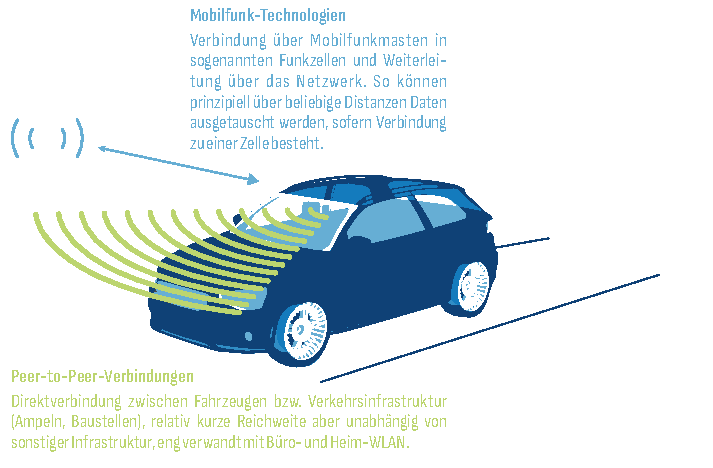
\includegraphics[width=12cm]{content/bottleneck/images/v2x-symbol4a.pdf}\hspace{-4cm}
		\end{tabular}
		
		Ein gegensätzliches Konzept sind die sogenannten \textbf{\color{colorKAMOLightGreen}Peer"=to"=Peer"=Verbindungen}, bei denen zwei Geräte in Reichweite eine direkte Verbindung aufnehmen, ohne einen zentralen Vermittler (das Mobilfunknetz) zu nutzen. Gängige Protokolle wie DSRC/WAVE bzw. ETSI ITS"=G5 (nicht mit >>5G<< zu verwechseln) sind eng verwandt mit dem WLAN bzw. Wi"=Fi, das in Büros, Heimnetzen und Hotspots genutzt wird. Sie alle setzen auf dem Funkstandard IEEE 802.11 auf. Die Reichweiten sind hier, ähnlich wie im privaten WLAN, eher kurz: Einige 100~m bis 1000~m können erreicht werden. Dafür funktioniert die Technik auch in Bereichen wo gar kein Mobilfunkempfang ist, wie entlegenen Regionen oder Tunnel.
		
		Und schließlich ist noch der zuvor genannte neue Mobilfunkstandard 5G noch einmal besonders zu erwähnen, da er zusätzlich auch Peer"=to"=Peer"=Verbindungen unterstützt.
		}
		\end{figure*}

\subsection{Gegenstand der Arbeiten}

Der >>vernetzte Engstellenassistent<< wurde im Projekt aus interdisziplinären Perspektiven betrachtet, um die Erfüllung der genannten Kriterien zu untersuchen. In der Publikation \cite{ehrhardt2021gap} wurden Aspekte der MMK im Fahrzeug und der Akzeptanz untersucht. In \cite{baumannbottleneck} wurden ausführlich die verkehrlichen Effekte des Systems analysiert. In \cite{Kowalewski2020_1000099791} wurden Untersuchungen mit neu entwickelten Richtantennensystemen durchgeführt, anhand derer sich abschätzen lässt, welche Kommunikationsreichweiten im urbanen Raum für vernetztes Fahren zu erwarten sind. Zudem wurden Befragungen zu Akzeptanz, sowie Kauf- und Nutzungsbereitschaft einer entsprechenden Funktion durchgeführt.

In diesem Beitrag konzentrieren wir uns hingegen auf die Frage, wie eine optimale Verhandlungsstrategie zwischen den vernetzten, kooperativen Fahrzeugen aussehen sollte, die sicherstellt, dass die Funktion für alle beteiligten Verkehrsteilnehmer akzeptabel ist, und insbesondere für die >>gewährenden<< Nutzer vermeidet, dass diese die Funktion einfach abschalten, um keine Nachteile in Kauf zu nehmen -- sowie die damit verbundene Frage, welche technischen Voraussetzungen notwendig sind, um das System zu realisieren. Um diese >>optimale Strategie<< zu finden, messen wir die Auswirkungen auf den Verkehrsfluss in umfangreichen Simulationsuntersuchungen und besprechen auffällige und interessante Effekte.

Dabei befassen wir uns spezifisch mit der Situation im \emph{dichten} Verkehr, in dem sich Warteschlangen bilden und deren Abfluss geregelt werden soll, ohne eine zentralisierte Steuerung (zum Beispiel eine Ampel) zu erfordern. Mit dem Fall von \emph{dünnem} Verkehr, in dem nur vereinzelt Fahrzeuge die Engtstelle passieren, befasst sich hingegen die Publikation \cite{naumann2017cooperativePlanning}.








		
		
\begin{figure*}%
\begin{thinmargin}
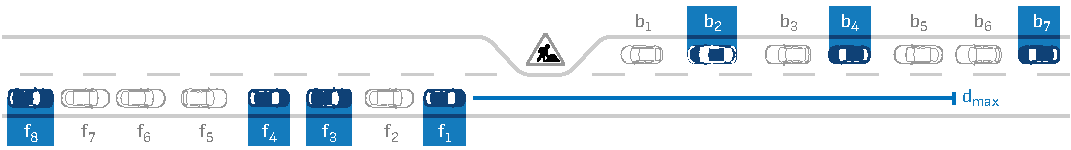
\includegraphics[width=\textwidth]{content/bottleneck/images/2021-bottleneck-paper}%
\caption{Beispielhafte Situation an der Engstelle, wobei Fahrzeuge mit der kooperativen Funktion blau gefüllt dargestellt sind, alle anderen (zum Beispiel menschlich gefahrene) Fahrzeuge als Umrisse. Die Fahrzeuge auf dem blockierten Streifen ($b_1, ..., b_7$) müssen darauf warten, dass eines der Fahrzeuge auf dem freien Streifen ($f_1, ..., f_8$) ihnen die Vorfahrt gewährt. Ziel war es, eine Methode zu finden, wie sich die kooperativen Fahrzeuge über Funk auf eine Strategie verständigen können. Die vorgeschlagene Lösung besteht darin, dass jedes kooperative Fahrzeug auf dem freien Streifen (genauer gesagt vermutlich: die Passagiere des jeweiligen Fahrzeugs) einen Wert $\dmax$ auswählen, der angibt, wie viele blockierte Fahrzeuge sie maximal abfließen lassen würden.}%
\label{fig:example}%
\end{thinmargin}
\end{figure*}


\subsection{Problemdefinition und Anforderungen}\label{sec:problem-definition}


Für eine zweistreifige Straße, wie in Abb.~\ref{fig:example} dargestellt, unterscheiden wir zwischen Fahrzeugen auf dem \emph{blockierten Streifen}, die an der Engstelle in den Gegenverkehr wechseln müssen, und Fahrzeugen auf dem \emph{freien Streifen}, die auf dem eigenen Streifen durch die Engstelle fahren können. Es sind keine Ampeln aufgebaut; es wird davon ausgegangen, dass gemäß Verkehrsregeln der \emph{freie Streifen} im Allgemeinen Vorfahrt hat, jedoch dem blockierten Streifen die Vorfahrt einräumen kann.

Wir bezeichnen die Fahrzeuge auf dem \emph{freien} sowie dem \emph{blockierten} Streifen mit
\begin{equation}
F = (f_1, f_2, f_3, ...)\;\;\text{bzw.}\;\; B = (b_1, b_2, b_3, ...).
\end{equation}
Da das System als Zusatzausstattung eines automatisierten Fahrzeugs konzipiert ist, können wir davon ausgehen, dass die nutzenden Fahrzeuge ohnehin über einen Grundstock von Technologie verfügen, die einen automatisierten Betrieb in der Umgebung ermöglicht. Konkret setzen wir voraus, dass die Fahrzeuge über folgende Technologie verfügen, die durch das kooperative System mitgenutzt werden kann:
\begin{itemize}
	\item Systeme für Umgebungswahrnehmung und automatisiertes Fahren, um die reguläre Fahraufgabe (ohne die neue vernetzte Funktion) bewältigen zu können. Dazu würde üblicherweise die Fähigkeit gehören, andere Verkehrsteilnehmer und befahrbare Straßenbereiche zu erkennen, sodass das Fahrzeug >>autonom<< durch die Engstelle fahren könnte, wenn der Verkehr das zulässt.
	
	%Die neue kooperative Funktion ist bewusst so gestaltet, dass sie diese sicherheitskritischen Funktionen nicht beeinträchtigen kann und keine spezifischen Annahmen trifft, wie diese funktionieren.
	\item Ein System zur globalen oder relativen Positionierung auf der Straße (bspw. GPS mit Kartendaten)
	\item Eine Technologie zur Kommunikation mit potentiellen Partnerfahrzeugen, entweder über Mobilfunk (4G, 5G) oder über lokale Direktverbindungen, wie die WLAN"=verwandten Standards 802.11p, DSRC/WAVE bzw. ETSI ITS"=G5.
\end{itemize}
Wir gehen außerdem davon aus, dass das System grob den Verlauf der Engstelle kennt, zum Beispiel dank anderer vernetzter Fahrzeuge, die sie bereits durchquert haben.



Aus verkehrlicher Sicht ist wünschenswert, dass sich ein >>ausgeglichener Fluss<< ergibt, also beide Richtungen gleichmäßig abfließen können.\footnote{Das ist tatsächlich etwas vereinfacht, weil es sein kann, dass in eine Richtung eine wesentlich höhere Nachfrage herrscht, beispielsweise zum Feierabend in Richtung Stadtauswärts, und sich entsprechend mehr Fahrzeuge in dieser Richtung stauen -- diese Unterscheidung ist aber hier nicht wesentlich.} Auf dieser Grundlage lassen sich die folgenden Anforderungen formulieren:
\begin{itemize}
	\item Verkehrsfluss sollte ausgeglichener werden, je mehr kooperative Fahrzeuge im Verkehr existieren
	\item Negative \emph{allgemeine} Effekte sollten vermieden werden: Das System sollte nicht >>überkompensieren<< und systematisch vernetzte Fahrzeuge, oder Fahrzeuge auf dem freien Streifen benachteiligen -- sowohl bei geringen Durchsetzungsquoten an kooperativen Fahrzeugen, wie auch im weit in der Zukunft liegenden Fall, wo potentiell alle Fahrzeuge ein entsprechendes System haben.
	\item Negative \emph{individuelle} Effekte für einzelne Verkehrsteilnehmer sollen konkret benannt und möglichst begrenzt werden.
	\item Technische Mehraufwände für die Umsetzung sollen vermieden werden; insbesondere soll keine zentrale, Ampel"=artige Steuerungsinstanz betrieben werden. Das System soll dezentral arbeiten können.
	\item Sicherheitskritische Funktionen des Fahrzeugs sollen nicht berührt werden.
\end{itemize}





\subsection{Der Kooperations"=Algorithmus}\label{sec:algorithm}

Basierend auf diesen Überlegungen soll nun ein Algorithmus entwickelt werden, anhand dessen sich die vernetzten Fahrzeuge in der Nähe einer Engstelle abstimmen können, und entscheiden, welches Fahrzeug unter welchen Bedingungen Vorfahrt gewährt -- und unter welchen nicht. Um unsere tatsächliche Lösung zu motivieren, lohnt es sich, einige Varianten zu diskutieren, die unsere Anforderungen \emph{nicht} geeignet erfüllen.

\subsubsection{Die nicht"=vernetzte Variante}

Prinzipiell lässt sich >>höfliches<< autonomes Fahren auch ohne Funk realisieren. Beispielsweise könnte ein automatisiertes Fahrzeug auf dem freien Streifen einfach nach Zufallsprinzip ab und zu die Vorfahrt gewähren (zum Beispiel indem es anhält und Lichthupe gibt). Das wäre ausreichend um zu einem ausgeglicheneren Verkehrsfluss beizutragen: Je mehr solcher Fahrzeuge im Verkehr sind, umso regelmäßiger wechselt der Verkehrsfluss die Richtung, und umso >>fairer<< der Fluss. Das Problem: Gewährt ein autonomes Fahrzeug auf dem freien Streifen die Vorfahrt, könnten auf dem blockierten Streifen beliebig viele Fahrzeuge abfließen. Die Passagiere des gewährenden Fahrzeugs müssten warten, bis auf dem blockierten Streifen wieder ein Fahrzeug die Vorfahrt zurückgibt. Diese Unwägbarkeit kann die Akzeptanz deutlich einschränken: Passagiere, die zum Beispiel pünktlich zu einer gegebenen Zeit am Ziel ankommen müssen, würden eine solche Funktion vermutlich ungern nutzen.

\subsubsection{Die >>ich"=möchte"=fahren<<-Variante}

Setzen wir nun voraus, dass Fahrzeuge über Funk kommunizieren können, ist das Naheliegendste, dass wartende Fahrzeuge auf dem blockierten Streifen eine Funknachricht absetzen, die besagt: >>Ich möchte fahren.<< Ein entsprechend ausgestattetes Fahrzeug auf dem freien Streifen könnte dann diesem Fahrzeug den Gefallen tun und die Vorfahrt gewähren. Aber diese Funknachricht ist im Grunde bedeutungslos: Alle Fahrzeuge auf dem freien Streifen können gesichert annehmen, dass alle Fahrzeuge auf dem blockierten Streifen (autonom, vernetzt oder einfach nur menschlich gesteuert) gerne abfließen wollen. Diese Variante bringt also praktisch keinen grundsätzlichen Vorteil gegenüber der nicht"=vernetzten Variante: %%, außer, dass sich ein Bonus für Nutzer eines kompatiblen Systems realisieren ließe. An dem Hauptproblem, dass
Das gewährende Fahrzeug müsste potentiell unkalkulierbar lange warten.


%\begin{mdframed}[linecolor=colorKAMOBlue] 
%%\fhmarginpar{Die Herausforderung besteht \emph{nicht} darin, eine passende Gelegenheit zum Vorfahrt"=Gewähren zu finden, sondern sicherzustellen, dass negative Effekte für alle beteiligten Verkehrsteilnehmer minimiert werden.}
%\end{mdframed}



\subsubsection{Die tatsächlich entwickelte Variante}\label{sec:var-proposed}

\fquot{}{Die Herausforderung besteht \emph{nicht} darin, eine passende Gelegenheit zum Vorfahrt"=Gewähren zu finden, sondern sicherzustellen, dass negative Effekte für alle beteiligten Verkehrsteilnehmer minimiert werden.}{}

Die tatsächlich entwickelte Variante ist in gewisser Weise das genaue Gegenteil der >>ich"=möchte"=Fahren<<-Variante: Fahrzeuge auf dem blockierten Streifen kommunizieren nicht ihren Fahrtwunsch, sondern ihre Bereitschaft, %\emph{nicht} in die Engstelle zu fahren sobald sie an der Spitze der Schlange ankommen. Sie erklären sich bereit,
vor der Engstelle zu halten und den Verkehrsfluss an den freien Streifen 3zurückzugeben. Warum sollten sie das tun, oder genauer: Kann es sein, dass alle Beteiligten davon profitieren?

Aus der Sicht von kooperativen Fahrzeugen auf dem freien Streifen ist der Vorteil klar: Wenn sie wissen, dass ein blockiertes Fahrzeug gesichert anhalten wird, können sie abschätzen, wie viel Zeit sie schlimmstenfalls verlieren. Haben sie noch ausreichend viel Zeitpuffer übrig, können sie die Vorfahrt gewähren und den Gegenverkehr bis zu diesem Fahrzeug abfließen lassen -- ansonsten tun sie das nicht. Konkret können die Passagiere in den Fahrzeugen auf dem freien Streifen einen Parameter $\dmax$ einstellen, der beispielsweise angibt, wie viele Fahrzeuge sie maximal abfließen lassen würden, wie in Abb.~\ref{fig:example} gezeigt. Findet sich ein vernetztes Fahrzeug auf dem blockierten Streifen, das maximal an Position $\dmax+1$ in der Warteschlange steht, gewährt das freie Fahrzeug der Gegenrichtung die Vorfahrt.\footnote{Tatsächlich ist es nicht ganz trivial, die Position in der Schlange zu bestimmen. Es würde sich also um einen ungefähren Schätzwert handeln, und es könnte auch eher eine geschätzte Wartezeit als eine Anzahl an Fahrzeugen sein. Die Erklärung des Prinzips würde das alles aber wesentlich verkomplizieren, deshalb gehen wir hier davon aus, dass die >>Anzahl an abfließenden Fahrzeugen<< hier die relevante und bekannte Maßeinheit ist.}

Aber auch das vernetzte Fahrzeug auf dem blockierten Streifen profitiert, obwohl es nur zusagt, \emph{nicht} zu fahren. Zwar wird es in dieser Runde sicherlich nicht die Engstelle durchqueren können, aber es rückt immerhin in der Schlange vor, dank seines Versprechens, zu warten. Sobald das nächste kooperative Fahrzeug an die freie Spitze kommt, kann es womöglich abfließen.

Wir schreiben >>womöglich<<, weil wir den Einfluss der menschlichen Fahrer nicht vergessen dürfen. Sie können sowohl auf dem freien Streifen höflich sein und ihrerseits (und zusätzlich) den blockierten Streifen abfließen lassen; es kann aber auch passieren, dass ein menschliches Fahrzeug auf dem blockierten Streifen stoppt und somit die Vorfahrt zurückgibt, bevor das kooperative Fahrzeug an der Spitze ankommt, das versprochen hatte, zu warten. In dem Fall fließen weniger als $\dmax$ Fahrzeuge vom blockierten Streifen ab; das dortige kooperative Fahrzeug rückt etwas vor, aber nicht bis an die Spitze. Diese Effekte werden wir berücksichtigen müssen. Gleichwohl gibt es kein (plausibles) Verhalten von menschlichen Fahrern, das den Sinn der Kooperation untergraben könnte.


Wir fassen den Abstimmungsprozess bis hierher kurz zusammen (Details sind der Original"=Publikation zu entnehmen):

\begin{enumerate}
	\item Ein kooperatives Fahrzeug auf dem freien Streifen $f_1$ nähert sich der Engstelle, und erkundigt sich nach Kooperationspartnern auf dem blockierten Streifen und ihren Warteschlangenpositionen. Zuvor (vermutlich zu Fahrtbeginn) haben die Passagiere von $f_1$ einen Parameter $\dmax$ gewählt.
	\item Alle kooperativen Fahrzeuge auf dem blockierten Streifen melden ihre Positionen zurück.
	\item Das Fahrzeug $f_1$ wählt dasjenige blockierte Fahrzeug aus, dessen Position \emph{höchstens} seinem $\dmax+1$ entspricht, und bittet dieses Fahrzeug, zu warten. In Abb.~\ref{fig:example} wäre das $b_4$.
	\item Stimmt dieses Fahrzeug ($b_4$) zu, gewährt $f_1$ dem blockierten Streifen die Vorfahrt: Es hält an und gibt Lichthupe. Außerdem benachrichtigt $f_1$ alle weiter vorne wartenden blockierten Fahrzeuge (in Abb.~\ref{fig:example} konkret $b_2$), dass sie ohne stoppen zu müssen abfließen dürfen.
	\item Sobald entweder ein menschlicherer Fahrer, oder das kooperative Partnerfahrzeug $b_4$ auf dem blockierten Streifen stoppen, kann $f_1$ in die Engstelle fahren.
\end{enumerate}

Ist das System so schon fertig? Nicht ganz: Auf dem blockierten Streifen sind jetzt (bis zu) $\dmax$ Fahrzeuge abgeflossen. Wenn jetzt direkt wieder ein kooperatives Fahrzeug auf dem freien Streifen kommt (in Abb.~\ref{fig:example} ist zum Beispiel das übernächste Fahrzeug $f_3$ wieder vernetzt, direkt gefolgt von einem weiteren, $f_4$), und alle diese Fahrzeuge wieder (bis zu) $\dmax$ Fahrzeuge abfließen lassen, kann es passieren, dass der freie Streifen plötzlich erheblich benachteiligt ist: Die vernetzten Fahrzeuge wären >>zu höflich<<, der Verkehrsfluss wäre überkompensiert. Genau das (unter anderem) wollen wir laut unseren Anforderungen vermeiden. Es muss sichergestellt werden, dass anschließend in etwa gleich viele Fahrzeuge auch vom freien Streifen abfließen wie vorher vom blockierten. Die menschlichen Fahrer auf dem freien Streifen können wir ebenso wenig beeinflussen wie die auf dem blockierten Streifen, aber wir können mit den vernetzten Fahrzeugen dort kommunizieren.

\begin{enumerate}[resume]
	\item Fahrzeug $f_1$ kommuniziert den nachfolgenden vernetzen Fahrzeugen (in Abb.~\ref{fig:example} $f_3$, $f_4$ und $f_8$), ... \fhmarginpar{Die >>zählende<< und die >>nicht"=zählende<< Variante}
	\begin{enumerate}
		\item \label{enum:non-counting}... entweder, dass alle Fahrzeuge bis Position $\dmax$ abfließen dürfen.
		\item \label{enum:counting} ... oder, dass alle Fahrzeuge bis $\dtats$ abfließen dürfen, wobei $\dtats$ die tatsächliche Anzahl an abgeflossenen Fahrzeugen ist (also weniger als $\dmax$, wenn ein menschliches Fahrzeug auf dem blockierten Streifen anhält).
	\end{enumerate}
\end{enumerate}

Welche der beiden Varianten ist besser? Macht das überhaupt einen Unterschied? Die zweite Frage ist eindeutig zu bejahen: Wir werden im folgenden Abschnitt \nameref{sec:evaluation} sehen, dass die verkehrlichen Effekte sich erheblich unterscheiden. Vorteilhaft in diesem Sinne ist Variante \ref{enum:counting}, die wir als >>zählende Variante<< bezeichnen werden. Allerdings ist das Zählen der abgeflossenen Fahrzeuge ein zusätzlicher technischer Aufwand, der mit dem Mehrwert abzuwägen ist.

\begin{figure}[t]%
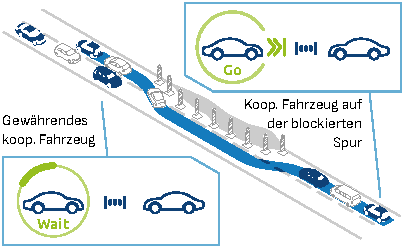
\includegraphics[width=\columnwidth]{content/bottleneck/images/engstelle-tuev-hmi-2}%
\caption{Beispiel der entwickelten Mensch"=Maschine"=Kommunikation (MMK), basierend auf \citep{ehrhardt2021gap}, wobei kooperative Fahrzeuge blau gefüllt dargestellt sind, alle anderen Fahrzeuge hingegen als Umrisse. Das vordere vernetzte Fahrzeug auf dem freien Streifen gewährt die Vorfahrt für den blockierte Streifen. Den Passagieren wird ein Countdown angezeigt, bis die Fahrt fortgesetzt wird. Das kommuniziert den Vorteil des Ansatzes, nämlich die klar abschätzbare maximale Wartedauer. Das kooperative Fahrzeug auf dem blockierten Streifen, das zugestimmt hat zu warten, zeigt seinen Passagieren den Fortschritt bis zur Spitze der Warteschlange an. Eine Untersuchung zur Wirkung einer möglichen MMK"=Gestaltung findet sich in \citep{ehrhardt2021gap}.}%
\label{fig:hmi}%
\end{figure}




Schließlich zeigt Abb.~\ref{fig:hmi} die entwickelte Mensch"=Maschine"=Kommunikation, die beispielsweise auf dem Display der beteiligten Fahrzeuge dargestellt werden kann (weitere Details siehe \cite{ehrhardt2021gap}). Sie ist danach ausgelegt, den Passagieren beider Fahrzeuge die Mehrwerte zu kommunizieren: Die Insassen des gewährenden Fahrzeugs auf dem freien Streifen erhalten eine konkrete Abschätzung der Wartedauer; die Insassen des Fahrzeugs, das schließlich an der Engstelle warten soll, erhalten eine Anzeige, wie sie in der Warteschlange aufrücken. Dies soll die Akzeptanz der Nutzung sicherstellen und damit die praktische Anwendbarkeit der Funktion.





\subsection{Evaluation}\label{sec:evaluation}

Während Teile des Systems auch in Realexperimenten untersuchbar sind, kann seine Wirkung im großflächigen, langfristigen Einsatz mit steigenden Durchsetzungsgraden von autonomen, kooperativen Fahrzeugen (also das, was uns besonders interessiert) nur in Simulationen studiert werden. Dabei gilt, dass jede Simulation nur Annahmen (sog. >>Modellannahmen<<) über die Realität abbildet. Entsprechend müssen diese Parameter gezielt auf die Fragestellung hin ausgewählt werden. Wir werden in den nachfolgenden Untersuchungen große Anzahlen an Verkehrsteilnehmern betrachten und viele Parameter variieren, sodass die Untersuchungen, grob abgeschätzt, die Messung von knapp 100 Jahren durchgängigen Verkehr abbilden.

\fquot{}{Grob abgeschätzt \textbf{100 Jahre} durchgängiger Verkehr wurden simuliert. Entsprechend reduziert muss die Komplexität der Simulation sein.}{}

Typische Simulationen im automatisierten Fahren beinhalten die Simulation von Umgebungssensoren, Fahrdynamik und detailliertem Verhalten menschlicher Verkehrsteilnehmer. Ein Simulationsschritt entspricht hier in der Regel Bruchteilen einer Sekunde. In diesem Detailgrad wäre eine entsprechend umfangreiche Untersuchung undenkbar -- wir müssen also die Komplexität drastisch reduzieren und nur das wesentliche Minimum an Details beibehalten.


%The system is described with software and V2V hardware setup with reference to close"=to"=marked automated vehicle equipment, and its properties are studied on driving simulations, human"=in"=the"=loop driving simulator studies and a consumer survey.

\begin{figure}
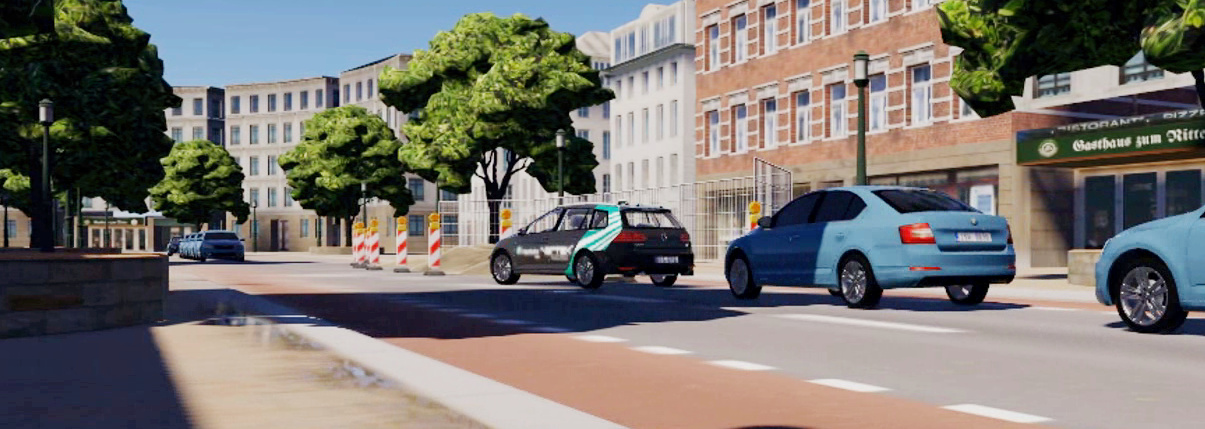
\includegraphics[width=\columnwidth]{content/bottleneck/images/octane-bottleneck}%
\caption[]{Bild der Szenariosimulation in OCTANE\footnotemark{} mit einer zweistreifigen Straße auf der eine Fahrtrichtung durch eine Baustelle blockiert ist. Die Fahrzeuge in dieser Richtung müssen in den Gegenverkehr wechseln. Im dichten Verkehr geht das nicht, ohne dass ein entgegenkommendes Fahrzeug die Vorfahrt gewährt.}%
\label{fig:octane}
\end{figure}
\footnotetext{\href{https://www.octane.org}{www.octane.org}}






\newcommand\carAny[1]{\colorbox{colorAny}{\!\textcolor{colorAny}{\texttt{00}}\!}}
\newcommand\carNum[1]{\colorbox{colorPRDGray}{\!\texttt{#1}\!}}
\newcommand\carFree[1]{\colorbox{colorPRMedBlue}{\!\texttt{\textcolor{white}{#1}}\!}}
\newcommand\carAgr[1]{\colorbox{colorPRDarkBlue}{\!\texttt{\textcolor{white}{#1}}\!}}


\newcommand\carAnyYield[1]{\colorbox{colorPRLightGreen}{\!\textcolor{colorPRLightGreen}{\texttt{00}}\!}}
\newcommand\carNumYield[1]{\colorbox{colorPRLightGreen}{\!\texttt{#1}\!}}


\newcommand\driveLeft{\quad\quad $\blacktriangleleft$\quad }
\newcommand\driveRight{\quad $\blacktriangleright$\quad\quad }
\newcommand\newlineCarPlot{\\[2pt]}

\newcounter{carplotline}

\newcommand\carPlotLine{\refstepcounter{carplotline}\noindent \llap{$\tau = \thecarplotline$}\; }

\begin{figure*}%
\begin{thinmargin}
\footnotesize
\begin{center}
freier Streifen (Zahlen zeigen gewähltes $\tdmax$) $\rightarrow$\hspace{0.2\textwidth}$\leftarrow$ blockierter Streifen (Zahlen zeigen Warteposition)
\end{center}
\begin{center}
\tiny
% \carPlotLine{}\carAny{--} \carAny{--} \carAny{--} \carAny{--} \carAny{--} \carAny{--} \carNum{07} \carAny{--} \carAny{--} \carAny{--} \carAny{--} \carNum{03} \carNum{02} \carAny{--} \carAny{--} \carNum{06} \carAny{--} \carAny{--} \carAny{--} \carAny{--} \driveRight{} \carAny{--} \carAny{--} \carNum{03} \carAny{--} \carAny{--} \carAny{--} \carNum{07} \carAny{--} \carAny{--} \carAny{--} \carAny{--} \carNum{12} \carAny{--} \carAny{--} \carAny{--} \carAny{--} \carNum{17} \carAny{--} \carAny{--} \carAny{--} \newlineCarPlot
% \carPlotLine{}\carAny{--} \carAny{--} \carAny{--} \carAny{--} \carAny{--} \carAny{--} \carAny{--} \carNum{07} \carAny{--} \carAny{--} \carAny{--} \carAny{--} \carNum{03} \carNum{02} \carAny{--} \carAny{--} \carNum{06} \carAny{--} \carAny{--} \carAny{--} \driveRight{} \carAny{--} \carAny{--} \carNum{03} \carAny{--} \carAny{--} \carAny{--} \carNum{07} \carAny{--} \carAny{--} \carAny{--} \carAny{--} \carNum{12} \carAny{--} \carAny{--} \carAny{--} \carAny{--} \carNum{17} \carAny{--} \carAny{--} \carAny{--} \newlineCarPlot
 \carPlotLine{}\carAny{--} \carAny{--} \carAny{--} \carAny{--} \carAny{--} \carAny{--} \carAny{--} \carAny{--} \carNum{07} \carAny{--} \carAny{--} \carAny{--} \carAny{--} \carNum{03} \carNum{02} \carAny{--} \carAny{--} \carNum{06} \carAny{--} \carAny{--} \driveRight{} \carAny{--} \carAny{--} \carNum{03} \carAny{--} \carAny{--} \carAny{--} \carNum{07} \carAny{--} \carAny{--} \carAny{--} \carAny{--} \carNum{12} \carAny{--} \carAny{--} \carAny{--} \carAny{--} \carNum{17} \carAny{--} \carAny{--} \carAny{--} \newlineCarPlot
 \carPlotLine{}\carNum{02} \carAny{--} \carAny{--} \carAny{--} \carAny{--} \carAny{--} \carAny{--} \carAny{--} \carAny{--} \carNum{07} \carAny{--} \carAny{--} \carAny{--} \carAny{--} \carNum{03} \carNum{02} \carAny{--} \carAny{--} \carNum{06} \carAny{--} \driveRight{} \carAny{--} \carAny{--} \carNum{03} \carAny{--} \carAny{--} \carAny{--} \carNum{07} \carAny{--} \carAny{--} \carAny{--} \carAny{--} \carNum{12} \carAny{--} \carAny{--} \carAny{--} \carAny{--} \carNum{17} \carAny{--} \carAny{--} \carAny{--} \newlineCarPlot
 \carPlotLine{}\carAny{--} \carNum{02} \carAny{--} \carAny{--} \carAny{--} \carAny{--} \carAny{--} \carAny{--} \carAny{--} \carAny{--} \carNum{07} \carAny{--} \carAny{--} \carAny{--} \carAny{--} \carNum{03} \carNum{02} \carAny{--} \carAny{--} \carNum{06} \driveRight{} \carAny{--} \carAny{--} \carNum{03} \carAny{--} \carAny{--} \carAny{--} \carNum{07} \carAny{--} \carAny{--} \carAny{--} \carAny{--} \carNum{12} \carAny{--} \carAny{--} \carAny{--} \carAny{--} \carNum{17} \carAny{--} \carAny{--} \carAny{--} \newlineCarPlot
 \carPlotLine{}\carAny{--} \carNum{02} \carAny{--} \carAny{--} \carAny{--} \carAny{--} \carAny{--} \carAny{--} \carAny{--} \carAny{--} \carNum{07} \carAny{--} \carAny{--} \carAny{--} \carAny{--} \carNum{03} \carNum{02} \carAny{--} \carAny{--} \carNumYield{06} \driveLeft{} \carAny{--} \carAny{--} \carFree{03} \carAny{--} \carAny{--} \carAny{--} \carAgr{07} \carAny{--} \carAny{--} \carAny{--} \carAny{--} \carNum{12} \carAny{--} \carAny{--} \carAny{--} \carAny{--} \carNum{17} \carAny{--} \carAny{--} \carAny{--} \newlineCarPlot
 \carPlotLine{}\carAny{--} \carNum{02} \carAny{--} \carAny{--} \carAny{--} \carAny{--} \carAny{--} \carAny{--} \carAny{--} \carAny{--} \carNum{07} \carAny{--} \carAny{--} \carAny{--} \carAny{--} \carNum{03} \carNum{02} \carAny{--} \carAny{--} \carNum{06} \driveLeft{} \carAny{--} \carFree{02} \carAny{--} \carAny{--} \carAny{--} \carAgr{06} \carAny{--} \carAny{--} \carAny{--} \carAny{--} \carNum{11} \carAny{--} \carAny{--} \carAny{--} \carAny{--} \carNum{16} \carAny{--} \carAny{--} \carAny{--} \carAny{--} \newlineCarPlot
 \carPlotLine{}\carAny{--} \carNum{02} \carAny{--} \carAny{--} \carAny{--} \carAny{--} \carAny{--} \carAny{--} \carAny{--} \carAny{--} \carNum{07} \carAny{--} \carAny{--} \carAny{--} \carAny{--} \carNum{03} \carNum{02} \carAny{--} \carAny{--} \carNum{06} \driveLeft{} \carFree{01} \carAny{--} \carAny{--} \carAny{--} \carAgr{05} \carAny{--} \carAny{--} \carAny{--} \carAny{--} \carNum{10} \carAny{--} \carAny{--} \carAny{--} \carAny{--} \carNum{15} \carAny{--} \carAny{--} \carAny{--} \carAny{--} \carAny{--} \newlineCarPlot
 \carPlotLine{}\carAny{--} \carNum{02} \carAny{--} \carAny{--} \carAny{--} \carAny{--} \carAny{--} \carAny{--} \carAny{--} \carAny{--} \carNum{07} \carAny{--} \carAny{--} \carAny{--} \carAny{--} \carNum{03} \carNum{02} \carAny{--} \carAny{--} \carNum{06} \driveLeft{} \carAny{--} \carAny{--} \carAny{--} \carAgr{04} \carAny{--} \carAny{--} \carAny{--} \carAny{--} \carNum{09} \carAny{--} \carAny{--} \carAny{--} \carAny{--} \carNum{14} \carAny{--} \carAny{--} \carAny{--} \carAny{--} \carAny{--} \carNum{20} \newlineCarPlot
 \carPlotLine{}\carAny{--} \carNum{02} \carAny{--} \carAny{--} \carAny{--} \carAny{--} \carAny{--} \carAny{--} \carAny{--} \carAny{--} \carNum{07} \carAny{--} \carAny{--} \carAny{--} \carAny{--} \carNum{03} \carNum{02} \carAny{--} \carAny{--} \carNum{06} \driveLeft{} \carAny{--} \carAny{--} \carAgr{03} \carAny{--} \carAny{--} \carAny{--} \carAny{--} \carNum{08} \carAny{--} \carAny{--} \carAny{--} \carAny{--} \carNum{13} \carAny{--} \carAny{--} \carAny{--} \carAny{--} \carAny{--} \carNum{19} \carAny{--} \newlineCarPlot
 \carPlotLine{}\carAny{--} \carNum{02} \carAny{--} \carAny{--} \carAny{--} \carAny{--} \carAny{--} \carAny{--} \carAny{--} \carAny{--} \carNum{07} \carAny{--} \carAny{--} \carAny{--} \carAny{--} \carNum{03} \carNum{02} \carAny{--} \carAny{--} \carNum{06} \driveLeft{} \carAny{--} \carAgr{02} \carAny{--} \carAny{--} \carAny{--} \carAny{--} \carNum{07} \carAny{--} \carAny{--} \carAny{--} \carAny{--} \carNum{12} \carAny{--} \carAny{--} \carAny{--} \carAny{--} \carAny{--} \carNum{18} \carAny{--} \carAny{--} \newlineCarPlot
 \carPlotLine{}\carAny{--} \carNum{02} \carAny{--} \carAny{--} \carAny{--} \carAny{--} \carAny{--} \carAny{--} \carAny{--} \carAny{--} \carNum{07} \carAny{--} \carAny{--} \carAny{--} \carAny{--} \carNum{03} \carNum{02} \carAny{--} \carAny{--} \carNum{06} \driveLeft{} \carAgr{01} \carAny{--} \carAny{--} \carAny{--} \carAny{--} \carNum{06} \carAny{--} \carAny{--} \carAny{--} \carAny{--} \carNum{11} \carAny{--} \carAny{--} \carAny{--} \carAny{--} \carAny{--} \carNum{17} \carAny{--} \carAny{--} \carAny{--} \newlineCarPlot
 \carPlotLine{}\carAny{--} \carNum{02} \carAny{--} \carAny{--} \carAny{--} \carAny{--} \carAny{--} \carAny{--} \carAny{--} \carAny{--} \carNum{07} \carAny{--} \carAny{--} \carAny{--} \carAny{--} \carNum{03} \carNum{02} \carAny{--} \carAny{--} \carFree{06} \driveRight{} \carNumYield{01} \carAny{--} \carAny{--} \carAny{--} \carAny{--} \carNum{06} \carAny{--} \carAny{--} \carAny{--} \carAny{--} \carNum{11} \carAny{--} \carAny{--} \carAny{--} \carAny{--} \carAny{--} \carNum{17} \carAny{--} \carAny{--} \carNum{20} \newlineCarPlot
 \carPlotLine{}\carNum{06} \carAny{--} \carNum{02} \carAny{--} \carAny{--} \carAny{--} \carAny{--} \carAny{--} \carAny{--} \carAny{--} \carAny{--} \carNum{07} \carAny{--} \carAny{--} \carAny{--} \carAny{--} \carFree{03} \carFree{02} \carAny{--} \carAny{--} \driveRight{} \carNum{01} \carAny{--} \carAny{--} \carAny{--} \carAny{--} \carNum{06} \carAny{--} \carAny{--} \carAny{--} \carAny{--} \carNum{11} \carAny{--} \carAny{--} \carAny{--} \carAny{--} \carAny{--} \carNum{17} \carAny{--} \carAny{--} \carNum{20} \newlineCarPlot
 \carPlotLine{}\carAny{--} \carNum{06} \carAny{--} \carNum{02} \carAny{--} \carAny{--} \carAny{--} \carAny{--} \carAny{--} \carAny{--} \carAny{--} \carAny{--} \carNum{07} \carAny{--} \carAny{--} \carAny{--} \carAny{--} \carFree{03} \carFree{02} \carAny{--} \driveRight{} \carNum{01} \carAny{--} \carAny{--} \carAny{--} \carAny{--} \carNum{06} \carAny{--} \carAny{--} \carAny{--} \carAny{--} \carNum{11} \carAny{--} \carAny{--} \carAny{--} \carAny{--} \carAny{--} \carNum{17} \carAny{--} \carAny{--} \carNum{20} \newlineCarPlot
 \carPlotLine{}\carAny{--} \carAny{--} \carNum{06} \carAny{--} \carNum{02} \carAny{--} \carAny{--} \carAny{--} \carAny{--} \carAny{--} \carAny{--} \carAny{--} \carAny{--} \carNum{07} \carAny{--} \carAny{--} \carAny{--} \carAny{--} \carFree{03} \carFree{02} \driveRight{} \carNum{01} \carAny{--} \carAny{--} \carAny{--} \carAny{--} \carNum{06} \carAny{--} \carAny{--} \carAny{--} \carAny{--} \carNum{11} \carAny{--} \carAny{--} \carAny{--} \carAny{--} \carAny{--} \carNum{17} \carAny{--} \carAny{--} \carNum{20} \newlineCarPlot
 \carPlotLine{}\carAny{--} \carAny{--} \carAny{--} \carNum{06} \carAny{--} \carNum{02} \carAny{--} \carAny{--} \carAny{--} \carAny{--} \carAny{--} \carAny{--} \carAny{--} \carAny{--} \carNum{07} \carAny{--} \carAny{--} \carAny{--} \carAny{--} \carFree{03} \driveRight{} \carNum{01} \carAny{--} \carAny{--} \carAny{--} \carAny{--} \carNum{06} \carAny{--} \carAny{--} \carAny{--} \carAny{--} \carNum{11} \carAny{--} \carAny{--} \carAny{--} \carAny{--} \carAny{--} \carNum{17} \carAny{--} \carAny{--} \carNum{20} \newlineCarPlot
 \carPlotLine{}\carAny{--} \carAny{--} \carAny{--} \carAny{--} \carNum{06} \carAny{--} \carNum{02} \carAny{--} \carAny{--} \carAny{--} \carAny{--} \carAny{--} \carAny{--} \carAny{--} \carAny{--} \carNum{07} \carAny{--} \carAny{--} \carAny{--} \carAny{--} \driveRight{} \carNum{01} \carAny{--} \carAny{--} \carAny{--} \carAny{--} \carNum{06} \carAny{--} \carAny{--} \carAny{--} \carAny{--} \carNum{11} \carAny{--} \carAny{--} \carAny{--} \carAny{--} \carAny{--} \carNum{17} \carAny{--} \carAny{--} \carNum{20} \newlineCarPlot
 \carPlotLine{}\carAny{--} \carAny{--} \carAny{--} \carAny{--} \carAny{--} \carNum{06} \carAny{--} \carNum{02} \carAny{--} \carAny{--} \carAny{--} \carAny{--} \carAny{--} \carAny{--} \carAny{--} \carAny{--} \carNum{07} \carAny{--} \carAny{--} \carAny{--} \driveRight{} \carNum{01} \carAny{--} \carAny{--} \carAny{--} \carAny{--} \carNum{06} \carAny{--} \carAny{--} \carAny{--} \carAny{--} \carNum{11} \carAny{--} \carAny{--} \carAny{--} \carAny{--} \carAny{--} \carNum{17} \carAny{--} \carAny{--} \carNum{20} \newlineCarPlot
 \carPlotLine{}\carAny{--} \carAny{--} \carAny{--} \carAny{--} \carAny{--} \carAny{--} \carNum{06} \carAny{--} \carNum{02} \carAny{--} \carAny{--} \carAny{--} \carAny{--} \carAny{--} \carAny{--} \carAny{--} \carAny{--} \carNum{07} \carAny{--} \carAny{--} \driveRight{} \carNum{01} \carAny{--} \carAny{--} \carAny{--} \carAny{--} \carNum{06} \carAny{--} \carAny{--} \carAny{--} \carAny{--} \carNum{11} \carAny{--} \carAny{--} \carAny{--} \carAny{--} \carAny{--} \carNum{17} \carAny{--} \carAny{--} \carNum{20} \newlineCarPlot
 \carPlotLine{}\carAny{--} \carAny{--} \carAny{--} \carAny{--} \carAny{--} \carAny{--} \carAny{--} \carNum{06} \carAny{--} \carNum{02} \carAny{--} \carAny{--} \carAny{--} \carAny{--} \carAny{--} \carAny{--} \carAny{--} \carAny{--} \carNum{07} \carAny{--} \driveRight{} \carNum{01} \carAny{--} \carAny{--} \carAny{--} \carAny{--} \carNum{06} \carAny{--} \carAny{--} \carAny{--} \carAny{--} \carNum{11} \carAny{--} \carAny{--} \carAny{--} \carAny{--} \carAny{--} \carNum{17} \carAny{--} \carAny{--} \carNum{20} \newlineCarPlot
 \carPlotLine{}\carAny{--} \carAny{--} \carAny{--} \carAny{--} \carAny{--} \carAny{--} \carAny{--} \carNum{06} \carAny{--} \carNum{02} \carAny{--} \carAny{--} \carAny{--} \carAny{--} \carAny{--} \carAny{--} \carAny{--} \carAny{--} \carNum{07} \carAnyYield{--} \driveLeft{} \carFree{01} \carAny{--} \carAny{--} \carAny{--} \carAny{--} \carNum{06} \carAny{--} \carAny{--} \carAny{--} \carAny{--} \carNum{11} \carAny{--} \carAny{--} \carAny{--} \carAny{--} \carAny{--} \carNum{17} \carAny{--} \carAny{--} \carNum{20} \newlineCarPlot
 \carPlotLine{}\carAny{--} \carAny{--} \carAny{--} \carAny{--} \carAny{--} \carAny{--} \carAny{--} \carNum{06} \carAny{--} \carNum{02} \carAny{--} \carAny{--} \carAny{--} \carAny{--} \carAny{--} \carAny{--} \carAny{--} \carAny{--} \carNum{07} \carAny{--} \driveLeft{} \carAny{--} \carAny{--} \carAny{--} \carAny{--} \carNum{05} \carAny{--} \carAny{--} \carAny{--} \carAny{--} \carNum{10} \carAny{--} \carAny{--} \carAny{--} \carAny{--} \carAny{--} \carNum{16} \carAny{--} \carAny{--} \carNum{19} \carAny{--} \newlineCarPlot
% \carPlotLine{}\carAny{--} \carAny{--} \carAny{--} \carAny{--} \carAny{--} \carAny{--} \carAny{--} \carNum{06} \carAny{--} \carNum{02} \carAny{--} \carAny{--} \carAny{--} \carAny{--} \carAny{--} \carAny{--} \carAny{--} \carAny{--} \carNum{07} \carAny{--} \driveLeft{} \carAny{--} \carAny{--} \carAny{--} \carNum{05} \carAny{--} \carAny{--} \carAny{--} \carAny{--} \carNum{10} \carAny{--} \carAny{--} \carAny{--} \carAny{--} \carAny{--} \carNum{16} \carAny{--} \carAny{--} \carNum{19} \carAny{--} \carAny{--} \newlineCarPlot
% \carPlotLine{}\carAny{--} \carAny{--} \carAny{--} \carAny{--} \carAny{--} \carAny{--} \carAny{--} \carNum{06} \carAny{--} \carNum{02} \carAny{--} \carAny{--} \carAny{--} \carAny{--} \carAny{--} \carAny{--} \carAny{--} \carAny{--} \carNum{07} \carAny{--} \driveLeft{} \carAny{--} \carAny{--} \carNum{04} \carAny{--} \carAny{--} \carAny{--} \carAny{--} \carNum{09} \carAny{--} \carAny{--} \carAny{--} \carAny{--} \carAny{--} \carNum{15} \carAny{--} \carAny{--} \carNum{18} \carAny{--} \carAny{--} \carAny{--} \newlineCarPlot
% \carPlotLine{}\carAny{--} \carAny{--} \carAny{--} \carAny{--} \carAny{--} \carAny{--} \carAny{--} \carNum{06} \carAny{--} \carNum{02} \carAny{--} \carAny{--} \carAny{--} \carAny{--} \carAny{--} \carAny{--} \carAny{--} \carAny{--} \carNum{07} \carAny{--} \driveLeft{} \carAny{--} \carNum{03} \carAny{--} \carAny{--} \carAny{--} \carAny{--} \carNum{08} \carAny{--} \carAny{--} \carAny{--} \carAny{--} \carAny{--} \carNum{14} \carAny{--} \carAny{--} \carNum{17} \carAny{--} \carAny{--} \carAny{--} \carAny{--} \newlineCarPlot
% \carPlotLine{}\carAny{--} \carAny{--} \carAny{--} \carAny{--} \carAny{--} \carAny{--} \carAny{--} \carNum{06} \carAny{--} \carNum{02} \carAny{--} \carAny{--} \carAny{--} \carAny{--} \carAny{--} \carAny{--} \carAny{--} \carAny{--} \carNum{07} \carAny{--} \driveLeft{} \carNum{02} \carAny{--} \carAny{--} \carAny{--} \carAny{--} \carNum{07} \carAny{--} \carAny{--} \carAny{--} \carAny{--} \carAny{--} \carNum{13} \carAny{--} \carAny{--} \carNum{16} \carAny{--} \carAny{--} \carAny{--} \carAny{--} \carAny{--} \newlineCarPlot
% \carPlotLine{}\carAny{--} \carAny{--} \carAny{--} \carAny{--} \carAny{--} \carAny{--} \carAny{--} \carNum{06} \carAny{--} \carNum{02} \carAny{--} \carAny{--} \carAny{--} \carAny{--} \carAny{--} \carAny{--} \carAny{--} \carAny{--} \carNum{07} \carAny{--} \driveRight{} \carNum{01} \carAny{--} \carAny{--} \carAny{--} \carAny{--} \carNum{06} \carAny{--} \carAny{--} \carAny{--} \carAny{--} \carAny{--} \carNum{12} \carAny{--} \carAny{--} \carNum{15} \carAny{--} \carAny{--} \carAny{--} \carAny{--} \carAny{--} \newlineCarPlot
% \carPlotLine{}\carAny{--} \carAny{--} \carAny{--} \carAny{--} \carAny{--} \carAny{--} \carAny{--} \carAny{--} \carNum{06} \carAny{--} \carNum{02} \carAny{--} \carAny{--} \carAny{--} \carAny{--} \carAny{--} \carAny{--} \carAny{--} \carAny{--} \carNum{07} \driveRight{} \carNum{01} \carAny{--} \carAny{--} \carAny{--} \carAny{--} \carNum{06} \carAny{--} \carAny{--} \carAny{--} \carAny{--} \carAny{--} \carNum{12} \carAny{--} \carAny{--} \carNum{15} \carAny{--} \carAny{--} \carAny{--} \carAny{--} \carAny{--} \newlineCarPlot
% \carPlotLine{}\carAny{--} \carAny{--} \carAny{--} \carAny{--} \carAny{--} \carAny{--} \carAny{--} \carAny{--} \carNum{06} \carAny{--} \carNum{02} \carAny{--} \carAny{--} \carAny{--} \carAny{--} \carAny{--} \carAny{--} \carAny{--} \carAny{--} \carNum{07} \driveLeft{} \carFree{01} \carAny{--} \carAny{--} \carAny{--} \carAny{--} \carAgr{06} \carAny{--} \carAny{--} \carAny{--} \carAny{--} \carAny{--} \carNum{12} \carAny{--} \carAny{--} \carNum{15} \carAny{--} \carAny{--} \carAny{--} \carAny{--} \carAny{--} \newlineCarPlot
% \carPlotLine{}\carAny{--} \carAny{--} \carAny{--} \carAny{--} \carAny{--} \carAny{--} \carAny{--} \carAny{--} \carNum{06} \carAny{--} \carNum{02} \carAny{--} \carAny{--} \carAny{--} \carAny{--} \carAny{--} \carAny{--} \carAny{--} \carAny{--} \carNum{07} \driveLeft{} \carAny{--} \carAny{--} \carAny{--} \carAny{--} \carAgr{06} \carAny{--} \carAny{--} \carAny{--} \carAny{--} \carAny{--} \carNum{12} \carAny{--} \carAny{--} \carNum{15} \carAny{--} \carAny{--} \carAny{--} \carAny{--} \carAny{--} \carAny{--} \newlineCarPlot
% \carPlotLine{}\carAny{--} \carAny{--} \carAny{--} \carAny{--} \carAny{--} \carAny{--} \carAny{--} \carAny{--} \carNum{06} \carAny{--} \carNum{02} \carAny{--} \carAny{--} \carAny{--} \carAny{--} \carAny{--} \carAny{--} \carAny{--} \carAny{--} \carNum{07} \driveLeft{} \carAny{--} \carAny{--} \carAny{--} \carAgr{05} \carAny{--} \carAny{--} \carAny{--} \carAny{--} \carAny{--} \carNum{11} \carAny{--} \carAny{--} \carNum{14} \carAny{--} \carAny{--} \carAny{--} \carAny{--} \carAny{--} \carAny{--} \carAny{--} \newlineCarPlot
% \carPlotLine{}\carAny{--} \carAny{--} \carAny{--} \carAny{--} \carAny{--} \carAny{--} \carAny{--} \carAny{--} \carNum{06} \carAny{--} \carNum{02} \carAny{--} \carAny{--} \carAny{--} \carAny{--} \carAny{--} \carAny{--} \carAny{--} \carAny{--} \carFree{07} \driveRight{} \carAny{--} \carAny{--} \carAny{--} \carAgr{04} \carAny{--} \carAny{--} \carAny{--} \carAny{--} \carAny{--} \carNum{10} \carAny{--} \carAny{--} \carNum{13} \carAny{--} \carAny{--} \carAny{--} \carAny{--} \carAny{--} \carAny{--} \carNum{20} \newlineCarPlot
% \carPlotLine{}\carNum{03} \carAny{--} \carAny{--} \carAny{--} \carAny{--} \carAny{--} \carAny{--} \carAny{--} \carAny{--} \carNum{06} \carAny{--} \carNum{02} \carAny{--} \carAny{--} \carAny{--} \carAny{--} \carAny{--} \carAny{--} \carAny{--} \carAny{--} \driveRight{} \carAny{--} \carAny{--} \carAny{--} \carNum{04} \carAny{--} \carAny{--} \carAny{--} \carAny{--} \carAny{--} \carNum{10} \carAny{--} \carAny{--} \carNum{13} \carAny{--} \carAny{--} \carAny{--} \carAny{--} \carAny{--} \carAny{--} \carNum{20} \newlineCarPlot
% \carPlotLine{}\carNum{03} \carAny{--} \carAny{--} \carAny{--} \carAny{--} \carAny{--} \carAny{--} \carAny{--} \carAny{--} \carNum{06} \carAny{--} \carNum{02} \carAny{--} \carAny{--} \carAny{--} \carAny{--} \carAny{--} \carAny{--} \carAny{--} \carAny{--} \driveLeft{} \carAny{--} \carAny{--} \carAny{--} \carNum{04} \carAny{--} \carAny{--} \carAny{--} \carAny{--} \carAny{--} \carNum{10} \carAny{--} \carAny{--} \carNum{13} \carAny{--} \carAny{--} \carAny{--} \carAny{--} \carAny{--} \carAny{--} \carNum{20} \newlineCarPlot
% \carPlotLine{}\carNum{03} \carAny{--} \carAny{--} \carAny{--} \carAny{--} \carAny{--} \carAny{--} \carAny{--} \carAny{--} \carNum{06} \carAny{--} \carNum{02} \carAny{--} \carAny{--} \carAny{--} \carAny{--} \carAny{--} \carAny{--} \carAny{--} \carAny{--} \driveLeft{} \carAny{--} \carAny{--} \carNum{04} \carAny{--} \carAny{--} \carAny{--} \carAny{--} \carAny{--} \carNum{10} \carAny{--} \carAny{--} \carNum{13} \carAny{--} \carAny{--} \carAny{--} \carAny{--} \carAny{--} \carAny{--} \carNum{20} \carAny{--} \newlineCarPlot
% \carPlotLine{}\carNum{03} \carAny{--} \carAny{--} \carAny{--} \carAny{--} \carAny{--} \carAny{--} \carAny{--} \carAny{--} \carNum{06} \carAny{--} \carNum{02} \carAny{--} \carAny{--} \carAny{--} \carAny{--} \carAny{--} \carAny{--} \carAny{--} \carAny{--} \driveLeft{} \carAny{--} \carNum{03} \carAny{--} \carAny{--} \carAny{--} \carAny{--} \carAny{--} \carNum{09} \carAny{--} \carAny{--} \carNum{12} \carAny{--} \carAny{--} \carAny{--} \carAny{--} \carAny{--} \carAny{--} \carNum{19} \carAny{--} \carAny{--} \newlineCarPlot
% \carPlotLine{}\carNum{03} \carAny{--} \carAny{--} \carAny{--} \carAny{--} \carAny{--} \carAny{--} \carAny{--} \carAny{--} \carNum{06} \carAny{--} \carNum{02} \carAny{--} \carAny{--} \carAny{--} \carAny{--} \carAny{--} \carAny{--} \carAny{--} \carAny{--} \driveLeft{} \carNum{02} \carAny{--} \carAny{--} \carAny{--} \carAny{--} \carAny{--} \carNum{08} \carAny{--} \carAny{--} \carNum{11} \carAny{--} \carAny{--} \carAny{--} \carAny{--} \carAny{--} \carAny{--} \carNum{18} \carAny{--} \carAny{--} \carAny{--} \newlineCarPlot
% \carPlotLine{}\carNum{03} \carAny{--} \carAny{--} \carAny{--} \carAny{--} \carAny{--} \carAny{--} \carAny{--} \carAny{--} \carNum{06} \carAny{--} \carNum{02} \carAny{--} \carAny{--} \carAny{--} \carAny{--} \carAny{--} \carAny{--} \carAny{--} \carAny{--} \driveRight{} \carNum{01} \carAny{--} \carAny{--} \carAny{--} \carAny{--} \carAny{--} \carNum{07} \carAny{--} \carAny{--} \carNum{10} \carAny{--} \carAny{--} \carAny{--} \carAny{--} \carAny{--} \carAny{--} \carNum{17} \carAny{--} \carAny{--} \carAny{--} \newlineCarPlot
% \carPlotLine{}\carNum{05} \carNum{03} \carAny{--} \carAny{--} \carAny{--} \carAny{--} \carAny{--} \carAny{--} \carAny{--} \carAny{--} \carNum{06} \carAny{--} \carNum{02} \carAny{--} \carAny{--} \carAny{--} \carAny{--} \carAny{--} \carAny{--} \carAny{--} \driveRight{} \carNum{01} \carAny{--} \carAny{--} \carAny{--} \carAny{--} \carAny{--} \carNum{07} \carAny{--} \carAny{--} \carNum{10} \carAny{--} \carAny{--} \carAny{--} \carAny{--} \carAny{--} \carAny{--} \carNum{17} \carAny{--} \carAny{--} \carAny{--} \newlineCarPlot
% \carPlotLine{}\carNum{06} \carNum{05} \carNum{03} \carAny{--} \carAny{--} \carAny{--} \carAny{--} \carAny{--} \carAny{--} \carAny{--} \carAny{--} \carNum{06} \carAny{--} \carNum{02} \carAny{--} \carAny{--} \carAny{--} \carAny{--} \carAny{--} \carAny{--} \driveRight{} \carNum{01} \carAny{--} \carAny{--} \carAny{--} \carAny{--} \carAny{--} \carNum{07} \carAny{--} \carAny{--} \carNum{10} \carAny{--} \carAny{--} \carAny{--} \carAny{--} \carAny{--} \carAny{--} \carNum{17} \carAny{--} \carAny{--} \carAny{--} \newlineCarPlot
% \carPlotLine{}\carAny{--} \carNum{06} \carNum{05} \carNum{03} \carAny{--} \carAny{--} \carAny{--} \carAny{--} \carAny{--} \carAny{--} \carAny{--} \carAny{--} \carNum{06} \carAny{--} \carNum{02} \carAny{--} \carAny{--} \carAny{--} \carAny{--} \carAny{--} \driveRight{} \carNum{01} \carAny{--} \carAny{--} \carAny{--} \carAny{--} \carAny{--} \carNum{07} \carAny{--} \carAny{--} \carNum{10} \carAny{--} \carAny{--} \carAny{--} \carAny{--} \carAny{--} \carAny{--} \carNum{17} \carAny{--} \carAny{--} \carAny{--} \newlineCarPlot
% \carPlotLine{}\carAny{--} \carAny{--} \carNum{06} \carNum{05} \carNum{03} \carAny{--} \carAny{--} \carAny{--} \carAny{--} \carAny{--} \carAny{--} \carAny{--} \carAny{--} \carNum{06} \carAny{--} \carNum{02} \carAny{--} \carAny{--} \carAny{--} \carAny{--} \driveRight{} \carNum{01} \carAny{--} \carAny{--} \carAny{--} \carAny{--} \carAny{--} \carNum{07} \carAny{--} \carAny{--} \carNum{10} \carAny{--} \carAny{--} \carAny{--} \carAny{--} \carAny{--} \carAny{--} \carNum{17} \carAny{--} \carAny{--} \carAny{--} \newlineCarPlot
% \carPlotLine{}\carAny{--} \carAny{--} \carAny{--} \carNum{06} \carNum{05} \carNum{03} \carAny{--} \carAny{--} \carAny{--} \carAny{--} \carAny{--} \carAny{--} \carAny{--} \carAny{--} \carNum{06} \carAny{--} \carNum{02} \carAny{--} \carAny{--} \carAny{--} \driveRight{} \carNum{01} \carAny{--} \carAny{--} \carAny{--} \carAny{--} \carAny{--} \carNum{07} \carAny{--} \carAny{--} \carNum{10} \carAny{--} \carAny{--} \carAny{--} \carAny{--} \carAny{--} \carAny{--} \carNum{17} \carAny{--} \carAny{--} \carAny{--} \newlineCarPlot
% \carPlotLine{}\carAny{--} \carAny{--} \carAny{--} \carAny{--} \carNum{06} \carNum{05} \carNum{03} \carAny{--} \carAny{--} \carAny{--} \carAny{--} \carAny{--} \carAny{--} \carAny{--} \carAny{--} \carNum{06} \carAny{--} \carNum{02} \carAny{--} \carAny{--} \driveRight{} \carNum{01} \carAny{--} \carAny{--} \carAny{--} \carAny{--} \carAny{--} \carNum{07} \carAny{--} \carAny{--} \carNum{10} \carAny{--} \carAny{--} \carAny{--} \carAny{--} \carAny{--} \carAny{--} \carNum{17} \carAny{--} \carAny{--} \carAny{--} \newlineCarPlot
% \carPlotLine{}\carAny{--} \carAny{--} \carAny{--} \carAny{--} \carAny{--} \carNum{06} \carNum{05} \carNum{03} \carAny{--} \carAny{--} \carAny{--} \carAny{--} \carAny{--} \carAny{--} \carAny{--} \carAny{--} \carNum{06} \carAny{--} \carNum{02} \carAny{--} \driveRight{} \carNum{01} \carAny{--} \carAny{--} \carAny{--} \carAny{--} \carAny{--} \carNum{07} \carAny{--} \carAny{--} \carNum{10} \carAny{--} \carAny{--} \carAny{--} \carAny{--} \carAny{--} \carAny{--} \carNum{17} \carAny{--} \carAny{--} \carAny{--} \newlineCarPlot
% \carPlotLine{}\carAny{--} \carAny{--} \carAny{--} \carAny{--} \carAny{--} \carAny{--} \carNum{06} \carNum{05} \carNum{03} \carAny{--} \carAny{--} \carAny{--} \carAny{--} \carAny{--} \carAny{--} \carAny{--} \carAny{--} \carNum{06} \carAny{--} \carNum{02} \driveRight{} \carNum{01} \carAny{--} \carAny{--} \carAny{--} \carAny{--} \carAny{--} \carNum{07} \carAny{--} \carAny{--} \carNum{10} \carAny{--} \carAny{--} \carAny{--} \carAny{--} \carAny{--} \carAny{--} \carNum{17} \carAny{--} \carAny{--} \carAny{--} \newlineCarPlot
% \carPlotLine{}\carAny{--} \carAny{--} \carAny{--} \carAny{--} \carAny{--} \carAny{--} \carAny{--} \carNum{06} \carNum{05} \carNum{03} \carAny{--} \carAny{--} \carAny{--} \carAny{--} \carAny{--} \carAny{--} \carAny{--} \carAny{--} \carNum{06} \carAny{--} \driveRight{} \carNum{01} \carAny{--} \carAny{--} \carAny{--} \carAny{--} \carAny{--} \carNum{07} \carAny{--} \carAny{--} \carNum{10} \carAny{--} \carAny{--} \carAny{--} \carAny{--} \carAny{--} \carAny{--} \carNum{17} \carAny{--} \carAny{--} \carAny{--} \newlineCarPlot
% \carPlotLine{}\carAny{--} \carAny{--} \carAny{--} \carAny{--} \carAny{--} \carAny{--} \carAny{--} \carAny{--} \carNum{06} \carNum{05} \carNum{03} \carAny{--} \carAny{--} \carAny{--} \carAny{--} \carAny{--} \carAny{--} \carAny{--} \carAny{--} \carNum{06} \driveRight{} \carNum{01} \carAny{--} \carAny{--} \carAny{--} \carAny{--} \carAny{--} \carNum{07} \carAny{--} \carAny{--} \carNum{10} \carAny{--} \carAny{--} \carAny{--} \carAny{--} \carAny{--} \carAny{--} \carNum{17} \carAny{--} \carAny{--} \carAny{--} \newlineCarPlot
% \carPlotLine{}\carAny{--} \carAny{--} \carAny{--} \carAny{--} \carAny{--} \carAny{--} \carAny{--} \carAny{--} \carNum{06} \carNum{05} \carNum{03} \carAny{--} \carAny{--} \carAny{--} \carAny{--} \carAny{--} \carAny{--} \carAny{--} \carAny{--} \carNum{06} \driveLeft{} \carFree{01} \carAny{--} \carAny{--} \carAny{--} \carAny{--} \carAny{--} \carAgr{07} \carAny{--} \carAny{--} \carNum{10} \carAny{--} \carAny{--} \carAny{--} \carAny{--} \carAny{--} \carAny{--} \carNum{17} \carAny{--} \carAny{--} \carAny{--} \newlineCarPlot
% \carPlotLine{}\carAny{--} \carAny{--} \carAny{--} \carAny{--} \carAny{--} \carAny{--} \carAny{--} \carAny{--} \carNum{06} \carNum{05} \carNum{03} \carAny{--} \carAny{--} \carAny{--} \carAny{--} \carAny{--} \carAny{--} \carAny{--} \carAny{--} \carNum{06} \driveLeft{} \carAny{--} \carAny{--} \carAny{--} \carAny{--} \carAny{--} \carAgr{07} \carAny{--} \carAny{--} \carNum{10} \carAny{--} \carAny{--} \carAny{--} \carAny{--} \carAny{--} \carAny{--} \carNum{17} \carAny{--} \carAny{--} \carAny{--} \carAny{--} \newlineCarPlot
% \carPlotLine{}\carAny{--} \carAny{--} \carAny{--} \carAny{--} \carAny{--} \carAny{--} \carAny{--} \carAny{--} \carNum{06} \carNum{05} \carNum{03} \carAny{--} \carAny{--} \carAny{--} \carAny{--} \carAny{--} \carAny{--} \carAny{--} \carAny{--} \carNum{06} \driveLeft{} \carAny{--} \carAny{--} \carAny{--} \carAny{--} \carAgr{06} \carAny{--} \carAny{--} \carNum{09} \carAny{--} \carAny{--} \carAny{--} \carAny{--} \carAny{--} \carAny{--} \carNum{16} \carAny{--} \carAny{--} \carAny{--} \carAny{--} \carAny{--} \newlineCarPlot
% \carPlotLine{}\carAny{--} \carAny{--} \carAny{--} \carAny{--} \carAny{--} \carAny{--} \carAny{--} \carAny{--} \carNum{06} \carNum{05} \carNum{03} \carAny{--} \carAny{--} \carAny{--} \carAny{--} \carAny{--} \carAny{--} \carAny{--} \carAny{--} \carNum{06} \driveLeft{} \carAny{--} \carAny{--} \carAny{--} \carAgr{05} \carAny{--} \carAny{--} \carNum{08} \carAny{--} \carAny{--} \carAny{--} \carAny{--} \carAny{--} \carAny{--} \carNum{15} \carAny{--} \carAny{--} \carAny{--} \carAny{--} \carAny{--} \carAny{--} \newlineCarPlot
% \carPlotLine{}\carAny{--} \carAny{--} \carAny{--} \carAny{--} \carAny{--} \carAny{--} \carAny{--} \carAny{--} \carNum{06} \carNum{05} \carNum{03} \carAny{--} \carAny{--} \carAny{--} \carAny{--} \carAny{--} \carAny{--} \carAny{--} \carAny{--} \carNum{06} \driveLeft{} \carAny{--} \carAny{--} \carAgr{04} \carAny{--} \carAny{--} \carNum{07} \carAny{--} \carAny{--} \carAny{--} \carAny{--} \carAny{--} \carAny{--} \carNum{14} \carAny{--} \carAny{--} \carAny{--} \carAny{--} \carAny{--} \carAny{--} \carAny{--} \newlineCarPlot
% \carPlotLine{}\carAny{--} \carAny{--} \carAny{--} \carAny{--} \carAny{--} \carAny{--} \carAny{--} \carAny{--} \carNum{06} \carNum{05} \carNum{03} \carAny{--} \carAny{--} \carAny{--} \carAny{--} \carAny{--} \carAny{--} \carAny{--} \carAny{--} \carNum{06} \driveLeft{} \carAny{--} \carAgr{03} \carAny{--} \carAny{--} \carNum{06} \carAny{--} \carAny{--} \carAny{--} \carAny{--} \carAny{--} \carAny{--} \carNum{13} \carAny{--} \carAny{--} \carAny{--} \carAny{--} \carAny{--} \carAny{--} \carAny{--} \carAny{--} \newlineCarPlot
% \carPlotLine{}\carAny{--} \carAny{--} \carAny{--} \carAny{--} \carAny{--} \carAny{--} \carAny{--} \carAny{--} \carNum{06} \carNum{05} \carNum{03} \carAny{--} \carAny{--} \carAny{--} \carAny{--} \carAny{--} \carAny{--} \carAny{--} \carAny{--} \carNum{06} \driveLeft{} \carAgr{02} \carAny{--} \carAny{--} \carNum{05} \carAny{--} \carAny{--} \carAny{--} \carAny{--} \carAny{--} \carAny{--} \carNum{12} \carAny{--} \carAny{--} \carAny{--} \carAny{--} \carAny{--} \carAny{--} \carAny{--} \carAny{--} \carAny{--} \newlineCarPlot
% \carPlotLine{}\carAny{--} \carAny{--} \carAny{--} \carAny{--} \carAny{--} \carAny{--} \carAny{--} \carAny{--} \carNum{06} \carNum{05} \carNum{03} \carAny{--} \carAny{--} \carAny{--} \carAny{--} \carAny{--} \carAny{--} \carAny{--} \carAny{--} \carFree{06} \driveRight{} \carAgr{01} \carAny{--} \carAny{--} \carNum{04} \carAny{--} \carAny{--} \carAny{--} \carAny{--} \carAny{--} \carAny{--} \carNum{11} \carAny{--} \carAny{--} \carAny{--} \carAny{--} \carAny{--} \carAny{--} \carAny{--} \carAny{--} \carAny{--} \newlineCarPlot
% \carPlotLine{}\carAny{--} \carAny{--} \carAny{--} \carAny{--} \carAny{--} \carAny{--} \carAny{--} \carAny{--} \carAny{--} \carNum{06} \carNum{05} \carNum{03} \carAny{--} \carAny{--} \carAny{--} \carAny{--} \carAny{--} \carAny{--} \carAny{--} \carAny{--} \driveRight{} \carNum{01} \carAny{--} \carAny{--} \carNum{04} \carAny{--} \carAny{--} \carAny{--} \carAny{--} \carAny{--} \carAny{--} \carNum{11} \carAny{--} \carAny{--} \carAny{--} \carAny{--} \carAny{--} \carAny{--} \carAny{--} \carAny{--} \carAny{--} \newlineCarPlot
% \carPlotLine{}\carAny{--} \carAny{--} \carAny{--} \carAny{--} \carAny{--} \carAny{--} \carAny{--} \carAny{--} \carAny{--} \carAny{--} \carNum{06} \carNum{05} \carNum{03} \carAny{--} \carAny{--} \carAny{--} \carAny{--} \carAny{--} \carAny{--} \carAny{--} \driveRight{} \carNum{01} \carAny{--} \carAny{--} \carNum{04} \carAny{--} \carAny{--} \carAny{--} \carAny{--} \carAny{--} \carAny{--} \carNum{11} \carAny{--} \carAny{--} \carAny{--} \carAny{--} \carAny{--} \carAny{--} \carAny{--} \carAny{--} \carAny{--} \newlineCarPlot
% \carPlotLine{}\carAny{--} \carAny{--} \carAny{--} \carAny{--} \carAny{--} \carAny{--} \carAny{--} \carAny{--} \carAny{--} \carAny{--} \carAny{--} \carNum{06} \carNum{05} \carNum{03} \carAny{--} \carAny{--} \carAny{--} \carAny{--} \carAny{--} \carAny{--} \driveRight{} \carNum{01} \carAny{--} \carAny{--} \carNum{04} \carAny{--} \carAny{--} \carAny{--} \carAny{--} \carAny{--} \carAny{--} \carNum{11} \carAny{--} \carAny{--} \carAny{--} \carAny{--} \carAny{--} \carAny{--} \carAny{--} \carAny{--} \carAny{--} \newlineCarPlot
% \carPlotLine{}\carAny{--} \carAny{--} \carAny{--} \carAny{--} \carAny{--} \carAny{--} \carAny{--} \carAny{--} \carAny{--} \carAny{--} \carAny{--} \carAny{--} \carNum{06} \carNum{05} \carNum{03} \carAny{--} \carAny{--} \carAny{--} \carAny{--} \carAny{--} \driveRight{} \carNum{01} \carAny{--} \carAny{--} \carNum{04} \carAny{--} \carAny{--} \carAny{--} \carAny{--} \carAny{--} \carAny{--} \carNum{11} \carAny{--} \carAny{--} \carAny{--} \carAny{--} \carAny{--} \carAny{--} \carAny{--} \carAny{--} \carAny{--} \newlineCarPlot
% \carPlotLine{}\carAny{--} \carAny{--} \carAny{--} \carAny{--} \carAny{--} \carAny{--} \carAny{--} \carAny{--} \carAny{--} \carAny{--} \carAny{--} \carAny{--} \carNum{06} \carNum{05} \carNum{03} \carAny{--} \carAny{--} \carAny{--} \carAny{--} \carAny{--} \driveLeft{} \carFree{01} \carAny{--} \carAny{--} \carNum{04} \carAny{--} \carAny{--} \carAny{--} \carAny{--} \carAny{--} \carAny{--} \carNum{11} \carAny{--} \carAny{--} \carAny{--} \carAny{--} \carAny{--} \carAny{--} \carAny{--} \carAny{--} \carAny{--} \newlineCarPlot
% \carPlotLine{}\carAny{--} \carAny{--} \carAny{--} \carAny{--} \carAny{--} \carAny{--} \carAny{--} \carAny{--} \carAny{--} \carAny{--} \carAny{--} \carAny{--} \carNum{06} \carNum{05} \carNum{03} \carAny{--} \carAny{--} \carAny{--} \carAny{--} \carAny{--} \driveLeft{} \carAny{--} \carAny{--} \carNum{04} \carAny{--} \carAny{--} \carAny{--} \carAny{--} \carAny{--} \carAny{--} \carNum{11} \carAny{--} \carAny{--} \carAny{--} \carAny{--} \carAny{--} \carAny{--} \carAny{--} \carAny{--} \carAny{--} \carAny{--} \newlineCarPlot
% \carPlotLine{}\carAny{--} \carAny{--} \carAny{--} \carAny{--} \carAny{--} \carAny{--} \carAny{--} \carAny{--} \carAny{--} \carAny{--} \carAny{--} \carAny{--} \carNum{06} \carNum{05} \carNum{03} \carAny{--} \carAny{--} \carAny{--} \carAny{--} \carAny{--} \driveLeft{} \carAny{--} \carNum{03} \carAny{--} \carAny{--} \carAny{--} \carAny{--} \carAny{--} \carAny{--} \carNum{10} \carAny{--} \carAny{--} \carAny{--} \carAny{--} \carAny{--} \carAny{--} \carAny{--} \carAny{--} \carAny{--} \carAny{--} \carAny{--} \newlineCarPlot
% \carPlotLine{}\carAny{--} \carAny{--} \carAny{--} \carAny{--} \carAny{--} \carAny{--} \carAny{--} \carAny{--} \carAny{--} \carAny{--} \carAny{--} \carAny{--} \carNum{06} \carNum{05} \carNum{03} \carAny{--} \carAny{--} \carAny{--} \carAny{--} \carAny{--} \driveLeft{} \carNum{02} \carAny{--} \carAny{--} \carAny{--} \carAny{--} \carAny{--} \carAny{--} \carNum{09} \carAny{--} \carAny{--} \carAny{--} \carAny{--} \carAny{--} \carAny{--} \carAny{--} \carAny{--} \carAny{--} \carAny{--} \carNum{20} \carAny{--} \newlineCarPlot
% \carPlotLine{}\carAny{--} \carAny{--} \carAny{--} \carAny{--} \carAny{--} \carAny{--} \carAny{--} \carAny{--} \carAny{--} \carAny{--} \carAny{--} \carAny{--} \carNum{06} \carNum{05} \carNum{03} \carAny{--} \carAny{--} \carAny{--} \carAny{--} \carAny{--} \driveRight{} \carNum{01} \carAny{--} \carAny{--} \carAny{--} \carAny{--} \carAny{--} \carAny{--} \carNum{08} \carAny{--} \carAny{--} \carAny{--} \carAny{--} \carAny{--} \carAny{--} \carAny{--} \carAny{--} \carAny{--} \carAny{--} \carNum{19} \carAny{--} \newlineCarPlot
% \carPlotLine{}\carAny{--} \carAny{--} \carAny{--} \carAny{--} \carAny{--} \carAny{--} \carAny{--} \carAny{--} \carAny{--} \carAny{--} \carAny{--} \carAny{--} \carAny{--} \carNum{06} \carNum{05} \carNum{03} \carAny{--} \carAny{--} \carAny{--} \carAny{--} \driveRight{} \carNum{01} \carAny{--} \carAny{--} \carAny{--} \carAny{--} \carAny{--} \carAny{--} \carNum{08} \carAny{--} \carAny{--} \carAny{--} \carAny{--} \carAny{--} \carAny{--} \carAny{--} \carAny{--} \carAny{--} \carAny{--} \carNum{19} \carAny{--} \newlineCarPlot
% \carPlotLine{}\carAny{--} \carAny{--} \carAny{--} \carAny{--} \carAny{--} \carAny{--} \carAny{--} \carAny{--} \carAny{--} \carAny{--} \carAny{--} \carAny{--} \carAny{--} \carAny{--} \carNum{06} \carNum{05} \carNum{03} \carAny{--} \carAny{--} \carAny{--} \driveRight{} \carNum{01} \carAny{--} \carAny{--} \carAny{--} \carAny{--} \carAny{--} \carAny{--} \carNum{08} \carAny{--} \carAny{--} \carAny{--} \carAny{--} \carAny{--} \carAny{--} \carAny{--} \carAny{--} \carAny{--} \carAny{--} \carNum{19} \carAny{--} \newlineCarPlot
% \carPlotLine{}\carAny{--} \carAny{--} \carAny{--} \carAny{--} \carAny{--} \carAny{--} \carAny{--} \carAny{--} \carAny{--} \carAny{--} \carAny{--} \carAny{--} \carAny{--} \carAny{--} \carAny{--} \carNum{06} \carNum{05} \carNum{03} \carAny{--} \carAny{--} \driveRight{} \carNum{01} \carAny{--} \carAny{--} \carAny{--} \carAny{--} \carAny{--} \carAny{--} \carNum{08} \carAny{--} \carAny{--} \carAny{--} \carAny{--} \carAny{--} \carAny{--} \carAny{--} \carAny{--} \carAny{--} \carAny{--} \carNum{19} \carAny{--} \newlineCarPlot
% \carPlotLine{}\carAny{--} \carAny{--} \carAny{--} \carAny{--} \carAny{--} \carAny{--} \carAny{--} \carAny{--} \carAny{--} \carAny{--} \carAny{--} \carAny{--} \carAny{--} \carAny{--} \carAny{--} \carAny{--} \carNum{06} \carNum{05} \carNum{03} \carAny{--} \driveRight{} \carNum{01} \carAny{--} \carAny{--} \carAny{--} \carAny{--} \carAny{--} \carAny{--} \carNum{08} \carAny{--} \carAny{--} \carAny{--} \carAny{--} \carAny{--} \carAny{--} \carAny{--} \carAny{--} \carAny{--} \carAny{--} \carNum{19} \carAny{--} \newlineCarPlot
% \carPlotLine{}\carNum{06} \carAny{--} \carAny{--} \carAny{--} \carAny{--} \carAny{--} \carAny{--} \carAny{--} \carAny{--} \carAny{--} \carAny{--} \carAny{--} \carAny{--} \carAny{--} \carAny{--} \carAny{--} \carAny{--} \carNum{06} \carNum{05} \carNum{03} \driveRight{} \carNum{01} \carAny{--} \carAny{--} \carAny{--} \carAny{--} \carAny{--} \carAny{--} \carNum{08} \carAny{--} \carAny{--} \carAny{--} \carAny{--} \carAny{--} \carAny{--} \carAny{--} \carAny{--} \carAny{--} \carAny{--} \carNum{19} \carAny{--} \newlineCarPlot
% \carPlotLine{}\carAny{--} \carNum{06} \carAny{--} \carAny{--} \carAny{--} \carAny{--} \carAny{--} \carAny{--} \carAny{--} \carAny{--} \carAny{--} \carAny{--} \carAny{--} \carAny{--} \carAny{--} \carAny{--} \carAny{--} \carAny{--} \carNum{06} \carNum{05} \driveRight{} \carNum{01} \carAny{--} \carAny{--} \carAny{--} \carAny{--} \carAny{--} \carAny{--} \carNum{08} \carAny{--} \carAny{--} \carAny{--} \carAny{--} \carAny{--} \carAny{--} \carAny{--} \carAny{--} \carAny{--} \carAny{--} \carNum{19} \carAny{--} \newlineCarPlot
% \carPlotLine{}\carAny{--} \carAny{--} \carNum{06} \carAny{--} \carAny{--} \carAny{--} \carAny{--} \carAny{--} \carAny{--} \carAny{--} \carAny{--} \carAny{--} \carAny{--} \carAny{--} \carAny{--} \carAny{--} \carAny{--} \carAny{--} \carAny{--} \carNum{06} \driveRight{} \carNum{01} \carAny{--} \carAny{--} \carAny{--} \carAny{--} \carAny{--} \carAny{--} \carNum{08} \carAny{--} \carAny{--} \carAny{--} \carAny{--} \carAny{--} \carAny{--} \carAny{--} \carAny{--} \carAny{--} \carAny{--} \carNum{19} \carAny{--} \newlineCarPlot
% \carPlotLine{}\carAny{--} \carAny{--} \carAny{--} \carNum{06} \carAny{--} \carAny{--} \carAny{--} \carAny{--} \carAny{--} \carAny{--} \carAny{--} \carAny{--} \carAny{--} \carAny{--} \carAny{--} \carAny{--} \carAny{--} \carAny{--} \carAny{--} \carAny{--} \driveRight{} \carNum{01} \carAny{--} \carAny{--} \carAny{--} \carAny{--} \carAny{--} \carAny{--} \carNum{08} \carAny{--} \carAny{--} \carAny{--} \carAny{--} \carAny{--} \carAny{--} \carAny{--} \carAny{--} \carAny{--} \carAny{--} \carNum{19} \carAny{--} \newlineCarPlot
% \carPlotLine{}\carAny{--} \carAny{--} \carAny{--} \carAny{--} \carNum{06} \carAny{--} \carAny{--} \carAny{--} \carAny{--} \carAny{--} \carAny{--} \carAny{--} \carAny{--} \carAny{--} \carAny{--} \carAny{--} \carAny{--} \carAny{--} \carAny{--} \carAny{--} \driveRight{} \carNum{01} \carAny{--} \carAny{--} \carAny{--} \carAny{--} \carAny{--} \carAny{--} \carNum{08} \carAny{--} \carAny{--} \carAny{--} \carAny{--} \carAny{--} \carAny{--} \carAny{--} \carAny{--} \carAny{--} \carAny{--} \carNum{19} \carAny{--} \newlineCarPlot
% \carPlotLine{}\carAny{--} \carAny{--} \carAny{--} \carAny{--} \carAny{--} \carNum{06} \carAny{--} \carAny{--} \carAny{--} \carAny{--} \carAny{--} \carAny{--} \carAny{--} \carAny{--} \carAny{--} \carAny{--} \carAny{--} \carAny{--} \carAny{--} \carAny{--} \driveRight{} \carNum{01} \carAny{--} \carAny{--} \carAny{--} \carAny{--} \carAny{--} \carAny{--} \carNum{08} \carAny{--} \carAny{--} \carAny{--} \carAny{--} \carAny{--} \carAny{--} \carAny{--} \carAny{--} \carAny{--} \carAny{--} \carNum{19} \carAny{--} \newlineCarPlot
% \carPlotLine{}\carAny{--} \carAny{--} \carAny{--} \carAny{--} \carAny{--} \carAny{--} \carNum{06} \carAny{--} \carAny{--} \carAny{--} \carAny{--} \carAny{--} \carAny{--} \carAny{--} \carAny{--} \carAny{--} \carAny{--} \carAny{--} \carAny{--} \carAny{--} \driveRight{} \carNum{01} \carAny{--} \carAny{--} \carAny{--} \carAny{--} \carAny{--} \carAny{--} \carNum{08} \carAny{--} \carAny{--} \carAny{--} \carAny{--} \carAny{--} \carAny{--} \carAny{--} \carAny{--} \carAny{--} \carAny{--} \carNum{19} \carAny{--} \newlineCarPlot
% \carPlotLine{}\carAny{--} \carAny{--} \carAny{--} \carAny{--} \carAny{--} \carAny{--} \carAny{--} \carNum{06} \carAny{--} \carAny{--} \carAny{--} \carAny{--} \carAny{--} \carAny{--} \carAny{--} \carAny{--} \carAny{--} \carAny{--} \carAny{--} \carAny{--} \driveRight{} \carNum{01} \carAny{--} \carAny{--} \carAny{--} \carAny{--} \carAny{--} \carAny{--} \carNum{08} \carAny{--} \carAny{--} \carAny{--} \carAny{--} \carAny{--} \carAny{--} \carAny{--} \carAny{--} \carAny{--} \carAny{--} \carNum{19} \carAny{--} \newlineCarPlot
% \carPlotLine{}\carAny{--} \carAny{--} \carAny{--} \carAny{--} \carAny{--} \carAny{--} \carAny{--} \carAny{--} \carNum{06} \carAny{--} \carAny{--} \carAny{--} \carAny{--} \carAny{--} \carAny{--} \carAny{--} \carAny{--} \carAny{--} \carAny{--} \carAny{--} \driveRight{} \carNum{01} \carAny{--} \carAny{--} \carAny{--} \carAny{--} \carAny{--} \carAny{--} \carNum{08} \carAny{--} \carAny{--} \carAny{--} \carAny{--} \carAny{--} \carAny{--} \carAny{--} \carAny{--} \carAny{--} \carAny{--} \carNum{19} \carAny{--} \newlineCarPlot
% \carPlotLine{}\carAny{--} \carAny{--} \carAny{--} \carAny{--} \carAny{--} \carAny{--} \carAny{--} \carAny{--} \carAny{--} \carNum{06} \carAny{--} \carAny{--} \carAny{--} \carAny{--} \carAny{--} \carAny{--} \carAny{--} \carAny{--} \carAny{--} \carAny{--} \driveRight{} \carNum{01} \carAny{--} \carAny{--} \carAny{--} \carAny{--} \carAny{--} \carAny{--} \carNum{08} \carAny{--} \carAny{--} \carAny{--} \carAny{--} \carAny{--} \carAny{--} \carAny{--} \carAny{--} \carAny{--} \carAny{--} \carNum{19} \carAny{--} \newlineCarPlot
% \carPlotLine{}\carAny{--} \carAny{--} \carAny{--} \carAny{--} \carAny{--} \carAny{--} \carAny{--} \carAny{--} \carAny{--} \carAny{--} \carNum{06} \carAny{--} \carAny{--} \carAny{--} \carAny{--} \carAny{--} \carAny{--} \carAny{--} \carAny{--} \carAny{--} \driveRight{} \carNum{01} \carAny{--} \carAny{--} \carAny{--} \carAny{--} \carAny{--} \carAny{--} \carNum{08} \carAny{--} \carAny{--} \carAny{--} \carAny{--} \carAny{--} \carAny{--} \carAny{--} \carAny{--} \carAny{--} \carAny{--} \carNum{19} \carAny{--} \newlineCarPlot
% \carPlotLine{}\carNum{05} \carAny{--} \carAny{--} \carAny{--} \carAny{--} \carAny{--} \carAny{--} \carAny{--} \carAny{--} \carAny{--} \carAny{--} \carNum{06} \carAny{--} \carAny{--} \carAny{--} \carAny{--} \carAny{--} \carAny{--} \carAny{--} \carAny{--} \driveRight{} \carNum{01} \carAny{--} \carAny{--} \carAny{--} \carAny{--} \carAny{--} \carAny{--} \carNum{08} \carAny{--} \carAny{--} \carAny{--} \carAny{--} \carAny{--} \carAny{--} \carAny{--} \carAny{--} \carAny{--} \carAny{--} \carNum{19} \carAny{--} \newlineCarPlot
% \carPlotLine{}\carAny{--} \carNum{05} \carAny{--} \carAny{--} \carAny{--} \carAny{--} \carAny{--} \carAny{--} \carAny{--} \carAny{--} \carAny{--} \carAny{--} \carNum{06} \carAny{--} \carAny{--} \carAny{--} \carAny{--} \carAny{--} \carAny{--} \carAny{--} \driveRight{} \carNum{01} \carAny{--} \carAny{--} \carAny{--} \carAny{--} \carAny{--} \carAny{--} \carNum{08} \carAny{--} \carAny{--} \carAny{--} \carAny{--} \carAny{--} \carAny{--} \carAny{--} \carAny{--} \carAny{--} \carAny{--} \carNum{19} \carAny{--} \newlineCarPlot
% \carPlotLine{}\carAny{--} \carNum{05} \carAny{--} \carAny{--} \carAny{--} \carAny{--} \carAny{--} \carAny{--} \carAny{--} \carAny{--} \carAny{--} \carAny{--} \carNum{06} \carAny{--} \carAny{--} \carAny{--} \carAny{--} \carAny{--} \carAny{--} \carAny{--} \driveLeft{} \carFree{01} \carAny{--} \carAny{--} \carAny{--} \carAny{--} \carAny{--} \carAny{--} \carNum{08} \carAny{--} \carAny{--} \carAny{--} \carAny{--} \carAny{--} \carAny{--} \carAny{--} \carAny{--} \carAny{--} \carAny{--} \carNum{19} \carAny{--} \newlineCarPlot
% \carPlotLine{}\carAny{--} \carNum{05} \carAny{--} \carAny{--} \carAny{--} \carAny{--} \carAny{--} \carAny{--} \carAny{--} \carAny{--} \carAny{--} \carAny{--} \carNum{06} \carAny{--} \carAny{--} \carAny{--} \carAny{--} \carAny{--} \carAny{--} \carAny{--} \driveLeft{} \carAny{--} \carAny{--} \carAny{--} \carAny{--} \carAny{--} \carAny{--} \carNum{08} \carAny{--} \carAny{--} \carAny{--} \carAny{--} \carAny{--} \carAny{--} \carAny{--} \carAny{--} \carAny{--} \carAny{--} \carNum{19} \carAny{--} \carAny{--} \newlineCarPlot
% \carPlotLine{}\carAny{--} \carNum{05} \carAny{--} \carAny{--} \carAny{--} \carAny{--} \carAny{--} \carAny{--} \carAny{--} \carAny{--} \carAny{--} \carAny{--} \carNum{06} \carAny{--} \carAny{--} \carAny{--} \carAny{--} \carAny{--} \carAny{--} \carAny{--} \driveRight{} \carAny{--} \carAny{--} \carAny{--} \carAny{--} \carAny{--} \carAny{--} \carNum{07} \carAny{--} \carAny{--} \carAny{--} \carAny{--} \carAny{--} \carAny{--} \carAny{--} \carAny{--} \carAny{--} \carAny{--} \carNum{18} \carAny{--} \carAny{--} \newlineCarPlot
% \carPlotLine{}\carAny{--} \carAny{--} \carNum{05} \carAny{--} \carAny{--} \carAny{--} \carAny{--} \carAny{--} \carAny{--} \carAny{--} \carAny{--} \carAny{--} \carAny{--} \carNum{06} \carAny{--} \carAny{--} \carAny{--} \carAny{--} \carAny{--} \carAny{--} \driveRight{} \carAny{--} \carAny{--} \carAny{--} \carAny{--} \carAny{--} \carAny{--} \carNum{07} \carAny{--} \carAny{--} \carAny{--} \carAny{--} \carAny{--} \carAny{--} \carAny{--} \carAny{--} \carAny{--} \carAny{--} \carNum{18} \carAny{--} \carAny{--} \newlineCarPlot
% \carPlotLine{}\carAny{--} \carAny{--} \carAny{--} \carNum{05} \carAny{--} \carAny{--} \carAny{--} \carAny{--} \carAny{--} \carAny{--} \carAny{--} \carAny{--} \carAny{--} \carAny{--} \carNum{06} \carAny{--} \carAny{--} \carAny{--} \carAny{--} \carAny{--} \driveRight{} \carAny{--} \carAny{--} \carAny{--} \carAny{--} \carAny{--} \carAny{--} \carNum{07} \carAny{--} \carAny{--} \carAny{--} \carAny{--} \carAny{--} \carAny{--} \carAny{--} \carAny{--} \carAny{--} \carAny{--} \carNum{18} \carAny{--} \carAny{--} \newlineCarPlot
% \carPlotLine{}\carAny{--} \carAny{--} \carAny{--} \carAny{--} \carNum{05} \carAny{--} \carAny{--} \carAny{--} \carAny{--} \carAny{--} \carAny{--} \carAny{--} \carAny{--} \carAny{--} \carAny{--} \carNum{06} \carAny{--} \carAny{--} \carAny{--} \carAny{--} \driveRight{} \carAny{--} \carAny{--} \carAny{--} \carAny{--} \carAny{--} \carAny{--} \carNum{07} \carAny{--} \carAny{--} \carAny{--} \carAny{--} \carAny{--} \carAny{--} \carAny{--} \carAny{--} \carAny{--} \carAny{--} \carNum{18} \carAny{--} \carAny{--} \newlineCarPlot
% \carPlotLine{}\carAny{--} \carAny{--} \carAny{--} \carAny{--} \carAny{--} \carNum{05} \carAny{--} \carAny{--} \carAny{--} \carAny{--} \carAny{--} \carAny{--} \carAny{--} \carAny{--} \carAny{--} \carAny{--} \carNum{06} \carAny{--} \carAny{--} \carAny{--} \driveRight{} \carAny{--} \carAny{--} \carAny{--} \carAny{--} \carAny{--} \carAny{--} \carNum{07} \carAny{--} \carAny{--} \carAny{--} \carAny{--} \carAny{--} \carAny{--} \carAny{--} \carAny{--} \carAny{--} \carAny{--} \carNum{18} \carAny{--} \carAny{--} \newlineCarPlot
% \carPlotLine{}\carAny{--} \carAny{--} \carAny{--} \carAny{--} \carAny{--} \carAny{--} \carNum{05} \carAny{--} \carAny{--} \carAny{--} \carAny{--} \carAny{--} \carAny{--} \carAny{--} \carAny{--} \carAny{--} \carAny{--} \carNum{06} \carAny{--} \carAny{--} \driveRight{} \carAny{--} \carAny{--} \carAny{--} \carAny{--} \carAny{--} \carAny{--} \carNum{07} \carAny{--} \carAny{--} \carAny{--} \carAny{--} \carAny{--} \carAny{--} \carAny{--} \carAny{--} \carAny{--} \carAny{--} \carNum{18} \carAny{--} \carAny{--} \newlineCarPlot
% \carPlotLine{}\carAny{--} \carAny{--} \carAny{--} \carAny{--} \carAny{--} \carAny{--} \carAny{--} \carNum{05} \carAny{--} \carAny{--} \carAny{--} \carAny{--} \carAny{--} \carAny{--} \carAny{--} \carAny{--} \carAny{--} \carAny{--} \carNum{06} \carAny{--} \driveRight{} \carAny{--} \carAny{--} \carAny{--} \carAny{--} \carAny{--} \carAny{--} \carNum{07} \carAny{--} \carAny{--} \carAny{--} \carAny{--} \carAny{--} \carAny{--} \carAny{--} \carAny{--} \carAny{--} \carAny{--} \carNum{18} \carAny{--} \carAny{--} \newlineCarPlot
% \carPlotLine{}\carAny{--} \carAny{--} \carAny{--} \carAny{--} \carAny{--} \carAny{--} \carAny{--} \carAny{--} \carNum{05} \carAny{--} \carAny{--} \carAny{--} \carAny{--} \carAny{--} \carAny{--} \carAny{--} \carAny{--} \carAny{--} \carAny{--} \carNum{06} \driveRight{} \carAny{--} \carAny{--} \carAny{--} \carAny{--} \carAny{--} \carAny{--} \carNum{07} \carAny{--} \carAny{--} \carAny{--} \carAny{--} \carAny{--} \carAny{--} \carAny{--} \carAny{--} \carAny{--} \carAny{--} \carNum{18} \carAny{--} \carAny{--} \newlineCarPlot
% \carPlotLine{}\carAny{--} \carAny{--} \carAny{--} \carAny{--} \carAny{--} \carAny{--} \carAny{--} \carAny{--} \carAny{--} \carNum{05} \carAny{--} \carAny{--} \carAny{--} \carAny{--} \carAny{--} \carAny{--} \carAny{--} \carAny{--} \carAny{--} \carAny{--} \driveRight{} \carAny{--} \carAny{--} \carAny{--} \carAny{--} \carAny{--} \carAny{--} \carNum{07} \carAny{--} \carAny{--} \carAny{--} \carAny{--} \carAny{--} \carAny{--} \carAny{--} \carAny{--} \carAny{--} \carAny{--} \carNum{18} \carAny{--} \carAny{--} \newlineCarPlot
% \carPlotLine{}\carAny{--} \carAny{--} \carAny{--} \carAny{--} \carAny{--} \carAny{--} \carAny{--} \carAny{--} \carAny{--} \carAny{--} \carNum{05} \carAny{--} \carAny{--} \carAny{--} \carAny{--} \carAny{--} \carAny{--} \carAny{--} \carAny{--} \carAny{--} \driveRight{} \carAny{--} \carAny{--} \carAny{--} \carAny{--} \carAny{--} \carAny{--} \carNum{07} \carAny{--} \carAny{--} \carAny{--} \carAny{--} \carAny{--} \carAny{--} \carAny{--} \carAny{--} \carAny{--} \carAny{--} \carNum{18} \carAny{--} \carAny{--} \newlineCarPlot
% \carPlotLine{}\carAny{--} \carAny{--} \carAny{--} \carAny{--} \carAny{--} \carAny{--} \carAny{--} \carAny{--} \carAny{--} \carAny{--} \carAny{--} \carNum{05} \carAny{--} \carAny{--} \carAny{--} \carAny{--} \carAny{--} \carAny{--} \carAny{--} \carAny{--} \driveRight{} \carAny{--} \carAny{--} \carAny{--} \carAny{--} \carAny{--} \carAny{--} \carNum{07} \carAny{--} \carAny{--} \carAny{--} \carAny{--} \carAny{--} \carAny{--} \carAny{--} \carAny{--} \carAny{--} \carAny{--} \carNum{18} \carAny{--} \carAny{--} \newlineCarPlot
% \carPlotLine{}\carNum{05} \carAny{--} \carAny{--} \carAny{--} \carAny{--} \carAny{--} \carAny{--} \carAny{--} \carAny{--} \carAny{--} \carAny{--} \carAny{--} \carNum{05} \carAny{--} \carAny{--} \carAny{--} \carAny{--} \carAny{--} \carAny{--} \carAny{--} \driveRight{} \carAny{--} \carAny{--} \carAny{--} \carAny{--} \carAny{--} \carAny{--} \carNum{07} \carAny{--} \carAny{--} \carAny{--} \carAny{--} \carAny{--} \carAny{--} \carAny{--} \carAny{--} \carAny{--} \carAny{--} \carNum{18} \carAny{--} \carAny{--}
\end{center}
\begin{tabular}{clclclcl}
\footnotesize
\carNum{XX}& koop. Fahrzeug &
\carFree{XX}& k.F. mit Fahrberechtigung&
\carAgr{XX}& \multicolumn{3}{l}{koop. Fahrzeug, das zugestimmt hat, zu warten}\\[5pt]
\carAny{00}& menschl. Fahrer&
\carAnyYield{00}& gewährendes Fhzg.&
$\blacktriangleright$& Fluss von freiem Streifen&
$\blacktriangleleft$& Fluss von blockiertem Streifen\\[5pt]
\multicolumn{8}{l}{Die Zahl \texttt{XX} gibt für Fahrzeuge im freien Streifen ihren gewählten $\tdmax$ an, im blockierten Streifen hingegen ihren Abstand $\tilde{d}$}
\end{tabular}
\caption[]{Auszug aus den simulierten Szenarien aus der rundenbasierten Perspektive, sodass ein Runde (Tau, $\tau$) hochgezählt wird, wenn ein Fahrzeug abfließt. Jede Kiste entspricht einem Fahrzeug. In der Darstellung >>verschwinden<< abgeflossene Fahrzeuge einfach in der Mitte, sodass je Streifen nur die wartenden Fahrzeuge gegenüberstehend dargestellt sind. Alle Fahrzeuge mit Nummern sind kooperative Fahrzeuge die das System nutzen; nicht nummerierte Fahrzeuge sind menschlich gesteuert (oder automatisiert aber ohne die kooperative Funktion). Die Nummern auf der linken Seite (freier Streifen) zeigen, wie viele entgegenkommende Fahrzeuge das vernetzte Fahrzeug maximal abfließen lassen würde, also $\tdmax$. Die Nummern auf der rechten Seite (blockierter Streifen) zeigen hingegen die Position in der Warteschlange an.\\[0.5em]
Das Szenario zeigt, dass ein kooperatives Fahrzeug in Runde $\tau = 3$ mit Einstellung $\tdmax=6$ Vorfahrt gewährt, weil das gegenüber wartende kooperative Fahrzeug mit $\tilde{d} = 7$ zugestimmt hat, zu warten. Somit ist sichergestellt, dass höchstens 6 Fahrzeuge abfließen. Es gibt noch ein näheres vernetztes Fahrzeug mit $\tilde{d} = 3$, das ausdrücklich die Erlaubnis erhält, abzufließen.  Alle menschlichen Fahrer auf dem blockierten Streifen fließen ab, das kooperative Fahrzeug hingegen wartet wie versprochen in Runde $\tau=10$, und gibt die Engstelle wieder für den freien Streifen frei. Das gewährende kooperative Fahrzeug auf dem freien Streifen fließt ab, und informiert die nachfolgenden vernetzten Fahrzeuge bis maximal zu Position 6, dass sie abfließen dürfen (praktisch ist das fernste Fahrzeug, das betroffen ist, aber nur 4 Positionen vom Kopf der Schlange entfernt).\\[0.5em]
Das vernetzte Fahrzeug vorn auf dem blockierten Streifen muss allerdings nicht auf das nächste vernetzte Fahrzeug warten: In Runde $\tau=20$ hält ein menschlicherer Fahrer auf dem freien Streifen an, und gewährt Vorfahrt. Damit kann das kooperative Fahrzeug abfließen.}%
\label{fig:scenario}%
\end{thinmargin}
\end{figure*}




\begin{figure*}[t!]%
\begin{thinmargin}
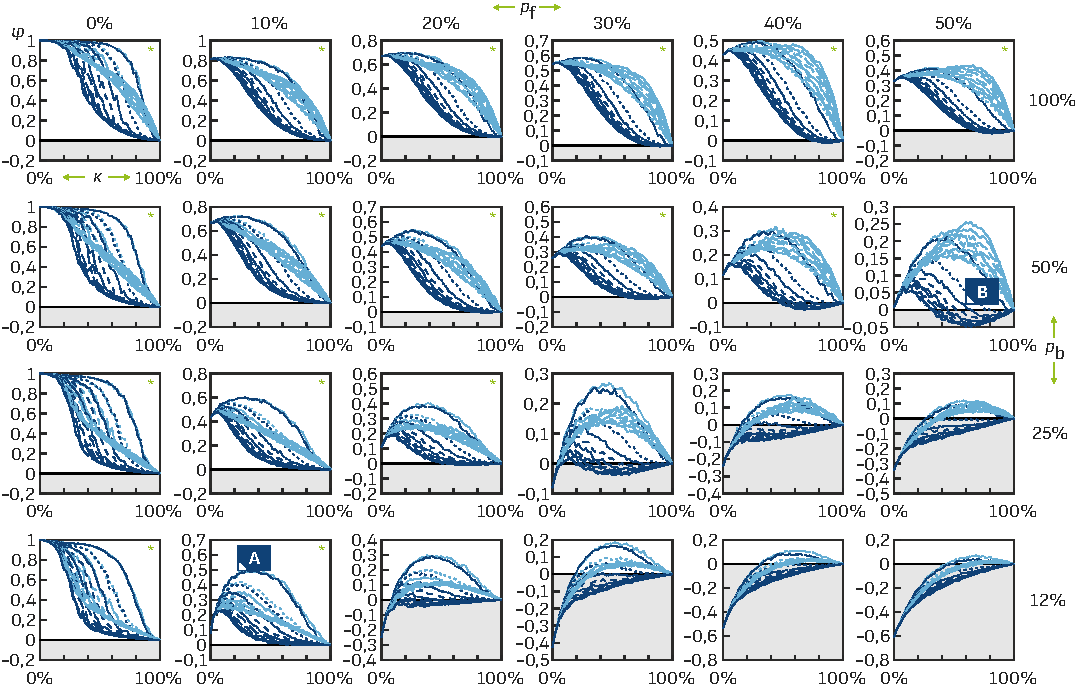
\includegraphics[width=\columnwidth]{content/bottleneck/images/tuev-engstelle-simulation-ergebnisse-7-kamo}%
\caption{Fluss"=Metrik $\varphi$ über unterschiedliche Durchsetzungsgrade kooperativer Fahrzeuge $\kappa$, aufgetragen über unterschiedliche menschliche Verhaltensparameter (die Wahrscheinlichkeit $p_{\text{f}}$ eines menschlichen Fahrers auf dem freien Streifen, die Vorfahrt zu gewähren, und die Wahrscheinlichkeit $p_{\text{b}}$ eines menschlichen Fahrers auf dem blockierten Streifen, die Vorfahrt zurückzugeben). Je durchgezogener eine Linie, umso höher der Kooperationsparameter $\tdmaxmax$. Hellblaue Linien beschreiben die >>nicht"=zählende<< Variante \ref{enum:non-counting} von Seite \pageref{enum:counting}, dunkelblaue Linien die >>zählende<< Variante \ref{enum:counting}. Im schattierten Bereich $\varphi < 0$ fließen sogar mehr Fahrzeuge vom blockierten Streifen ab, als vom freien Streifen. Nicht alle Parameterkombinationen sind dabei sehr wahrscheinlich. Die >>wahrscheinlicheren<< Parameterkombinationen, nämlich die wo Fahrer auf dem freien Streifen selbstbewusster fahren als Fahrer auf dem blockierten Streifen (in unserer Notation: $p\subs{f} < p\subs{b}$), sind mit einem grünen Sternchen \textcolor{colorPRGreen}{$*$} markiert. Auf diese kommen wir in Abb.~\ref{fig:simparameterresults-accumulated} noch einmal zurück.}%
\label{fig:simparameterresults}%
\end{thinmargin}
\end{figure*}












%The system was evaluated in a traffic simulation with different parameters for human behavior, different CAV algorithm designs, and different penetrations of compatible CAVs among other traffic participants. In each case, the scenario was a two"=way street with one lane in each direction (cf. Fig.~\ref{fig:octane})---one blocked by a construction site, the other free. Traffic volume was taken to be so high that negotiation between vehicles on opposite sides of the bottleneck was always required, to assure that the negotiation algorithm is always active in the results. The simulation only differentiates between compatible CAVs and >>other<< traffic participants, with no distinction between human drivers and non"=cooperative AVs.


\subsubsection{Grundprinzip des Simulationsaufbaus}

Die erste Vereinfachung besteht darin, einen Simulationsschritt nicht mehr als festen >>Sekundenbruchteil<< (bspw. $\nicefrac{1}{10}$ Sekunde) zu definieren: Stattdessen ist ein Schritt der Simulation immer das Abfließen eines einzelnen Fahrzeugs von einem der beiden Streifen. Wir nummerieren die Schritte mit dem Buchstaben Tau ($\tau$) (von engl. >>Turn<<, dt. >>Runde<<, >>Spielzug<<) wie in Abb.~\ref{fig:scenario} gezeigt.

Die detaillierten Fahrbewegungen zwischen den Runden werden nicht berücksichtigt. Wir betrachten außerdem (ebenfalls in Abb.~\ref{fig:scenario}) nur die wartenden Fahrzeuge. Sobald ein Fahrzeug abgeflossen ist, verschwindet es sofort aus der Simulation, weil es keinen relevanten Einfluss mehr hat. Wir betrachten jedes Szenario über $50\,000$ solcher >>Runden<<, was grob geschätzt drei Tagen Realverkehr an der Engstelle entsprechen würde.

Jedes Szenario hängt außerdem wesentlich von menschlichen Verhaltensweisen ab. Wie höflich fahren die Menschen schon selbst? Was für Kooperationsparameter $\tdmax$ wählen die Insassen eines vernetzten Fahrzeugs typischerweise? Das lässt sich heute unmöglich zuverlässig abschätzen und wird sicherlich auch zeitlich und regional stark variieren. Deshalb wählen wir den Ansatz, >>alle<< Parameterkombinationen durchzuprobieren. >>Alle<< in Anführungszeichen, weil das eine unendliche Menge wäre -- wir tasten in Wirklichkeit nur eine Auswahl an Parametern ab. Aber der Ansatz erlaubt es uns, viele mögliche Konstellationen auszuprobieren, sodass die tatsächliche Realität sich irgendwo durch die Parameterräume entwickeln wird. Vereinfacht gesagt: Wir wissen nicht, wie die Zukunft sich entwickelt, aber wir sind optimistisch, sie (näherungsweise) durch die Simulation abgedeckt zu haben. Damit sind die Ergebnisse der Studie aber deutlich weniger abhängig von sehr zugeschnittenen Annahmen, anhand derer zum Beispiel ein Realversuch durchführbar wäre (innerhalb dessen mit Sicherheit nicht circa 100 Jahre Verkehr untersucht würden).

Schauen wir uns also an, welche Parameter wir in der Simulation variieren, genauer gesagt: Welche >>Szenarioparameter<<  wir einstellen, um ein einzelnes Mal die besagten $50\,000$ Runden bzw. drei Tage Verkehr zu simulieren.

\fquot{}{Wir kennen die Zukunft nicht, aber wir sind optimistisch, sie (näherungsweise) durch die Simulation abgedeckt zu haben.}{}



\subsubsection{Simulationsparameter}

\paragraph{Die vernetzten Fahrzeuge} Die vernetzten Fahrzeuge verhalten sich entsprechend der vorgeschlagenen Funktion, wobei wir (wie auf Seite \pageref{enum:counting} diskutiert) zwischen der >>zählenden<< Variante \ref{enum:counting} und der >>nicht"=zählenden<< Variante \ref{enum:non-counting} unterscheiden. Basierend auf der Untersuchung von Funkreichweiten in \cite{Kowalewski2020_1000099791} nehmen wir an, dass Fahrzeuge über bis zu 20 Warteschlangenpositionen noch miteinander kommunizieren können, was in etwa 150\,m zuzüglich der Länge der Baustelle entspricht, und wir gehen davon aus, dass die Kommunikation so robust ist, dass der (relativ simple) Datenaustausch auf dieser Distanz nicht nennenswert gestört ist. Zum Kooperationsparameter $\tdmax$ nehmen wir an, dass die menschlichen Insassen ihn zufällig und gleichverteilt wählen zwischen 1 und einem Szenarioparameter, $\tdmaxmax$. Dieser Parameter $\tdmaxmax$ erlaubt es uns, gezielt Simulationsszenarien zu erzeugen, in denen die Insassen der vernetzten Fahrzeuge sehr großzügig sind (großes $\tdmaxmax$) oder sehr ungeduldig (kleines $\tdmaxmax$). In Formeln:
\begin{equation}
\begin{aligned}
\tdmax &\sim \mathcal{U}_{\mathbb N}(1, \tdmaxmax)\quad\text{and}\\
\tdmaxmax &\in \{4, 6, 8, ..., 20\}.
\end{aligned}
%\label{eq:}
\end{equation}

Wir gehen davon aus, dass im angenommenen dichten Verkehr die Funktion immer aktiv ist und das vernetzte Fahrverhalten vollständig beschreibt.


\paragraph{Alle anderen Fahrzeuge} Alle Fahrzeuge, die das vorgeschlagene System nicht nutzen, werden in einem stochastischen, also zufallsbasierten Modell zusammengefasst. Das können (in der Realität) menschlich gesteuerte Fahrzeuge sein, aber womöglich auch autonome Fahrzeuge ohne vernetzte Funktionen, oder sogar passende vernetzte Fahrzeuge, bei denen die Insassen die Funktion aber ausgeschaltet haben. Wir unterscheiden hier nicht weiter, sondern gehen davon aus, dass diese >>anderen<< Fahrzeuge sich stochastisch verhalten.

Das menschliche Verhalten hat für uns zwei Szenarioparameter: Die Wahrscheinlichkeit $p\subs{f}$ (zwischen $0\,\%$ und $100\,\%$), dass ein menschlicherer Fahrer auf dem freien Streifen anhält und den Gegenverkehr abfließen lässt; und die Wahrscheinlichkeit $p\subs{b}$, dass ein Fahrzeug auf dem blockierten Streifen anhält und die Vorfahrt zurückgibt (anstatt beim Abfließen dem Vorderfahrzeug in die Engstelle zu folgen). Wir gehen davon aus, dass bei einem Wechsel der Vorfahrt (ein Fahrzeug hält an und gewährt die Vorfahrt) das jeweils erste gegenüberliegende Fahrzeug mit absoluter Sicherheit abfließt. Die stochastischen Modelle beziehen sich also nur auf die nachfolgenden Fahrzeuge.

Die variierten Parameter (wie in Abb.~\ref{fig:simparameterresults}) sind
\begin{equation}
\begin{aligned}
p\subs{f} &\in \{0\,\%, 10\,\%, 20\,\%, 30\,\%, 40\,\%, 50\,\%\}\quad\text{und}\\
p\subs{b} &\in \{12\,\%, 25\,\%, 50\,\%, 100\,\%\}
\end{aligned}
%\label{eq:}
\end{equation}

\paragraph{Gesamtsimulation} In der Simulation werden unterschiedliche Durchsetzungsgrade $\kappa$ ausprobiert, mit
\begin{align}
\kappa &= \frac{\text{Anzahl vernetzter Fhzg.}}{\text{Anzahl aller Fhzg.}}\\[4pt]
\kappa &\in \{0\,\%, 2\,\%, 4\,\%, ..., 98\,\%, 100\,\%\},
\end{align}
wobei $\kappa = 0\,\%$ dem heutigen Verkehr ohne entsprechend vernetzte Fahrzeuge bezeichnet.

Damit können wir die Anzahl an Parameterkombinationen ausrechnen als
\begin{equation}
N\subs{Parameter} = N_{\tdmaxmax} \times N_{p\subs{f}} \times N_{p\subs{b}} \times N_\kappa = 11\,016\;,
\end{equation}
und jede dieser Kombinationen wird über die besagten 50\,000 Runden simuliert.



Jetzt fehlt noch ein Bewertungsmaßstab für jeden dieser Simulationsdurchläufe. Wir bewerten die >>Fairness<< des Verkehrsflusses in einem Szenario anhand der folgendermaßen definierten Fluss"=Metrik >>Phi<< ($\varphi$):
%\begin{equation}
%\varphi = 2 \cdot \frac{\text{\parbox{3cm}{\centering\setstretch{0.9} Anzahl der abgeflossenen Fahrzeuge auf dem freien Streifen \vspace{0.5em}}}}{\text{\parbox{3cm}{\vspace{0.5em}\centering\setstretch{0.9} Anzahl aller abgeflossenen Fahrzeuge}}} - 1
%\label{eq:}
%\end{equation}
%\begin{equation}
%\varphi =\frac{|\,\text{drained free vehs.}\,| - |\,\text{drained blocked vehs.}|\,}{|\,\text{all drained vehicles}\,|}
%\label{eq:}
%\end{equation}

\begin{equation}
\varphi = \frac{\left(\text{\parbox{1.7cm}{\centering\setstretch{0.9} Anzahl abgeflossener Fahrzeuge auf freiem Streifen\vspace{0.5em}}}\right) - \left(\text{\parbox{2cm}{\centering\setstretch{0.9} Anzahl abgeflossener Fahrzeuge auf blockiertem Streifen\vspace{0.5em}}}\right)}{\text{\parbox{4.5cm}{\vspace{0.5em}\centering\setstretch{0.9} Gesamtzahl aller abgeflossenen Fahrzeuge}}}
\end{equation}

Nach dieser Berechnung bedeutet ein Wert von $\varphi = 1$, dass über den betrachteten Zeitraum nur Fahrzeuge vom freien Streifen abfließen; bei $\varphi = 0$ herrscht ein ausgeglichener Fluss. Für $\varphi = -1$ fließen nur Fahrzeuge vom blockierten Streifen ab -- in der Praxis ein sehr unüblicher Zustand, den wir auch in unseren Experimenten nicht erreichen (und nicht erreichen wollen).


\subsubsection{Ergebnisse}

Die Ergebnisse der Simulationsuntersuchungen sind in Abb.~\ref{fig:simparameterresults} gezeigt (aufgeschlüsselt nach allen Szenarioparametern), sowie in Abb.~\ref{fig:simparameterresults-accumulated} (gemittelt über die >>wahrscheinlicheren<< Parameter). Wir können in diesen Ergebnissen einige sehr interessante Effekte beobachten, die Rückschlüsse über unsere Funktion und sinnvolle Realisierungen geben.

Zuerst können wir sehen, dass jede Variante der Wunschzustand $\varphi \rightarrow 0$ erreicht, wenn der Anteil der vernetzten Fahrzeuge bis zur vollständigen Durchsetzung ansteigt $\kappa \rightarrow 100\,\%$. Das bedeutet: Der Algorithmus kann >>evolutionär<< funktionieren und wird besser (statt schlechter) je mehr entsprechende Fahrzeuge im Verkehr sind. Das ist gut, so war es gedacht. Wir können auch sehen, dass die menschlichen Verhaltensparameter einen erheblichen Einfluss haben darauf, wie schnell der Verkehr mit zunehmenden Durchsetzungsgraden >>fairer<< wird.

Es gibt aber auch einige zunächst paradox wirkende Effekte, die nicht dem entsprechen, was man zuerst erwartet hättet. Eine vollständige Diskussion findet sich in der Originalpublikation, wir greifen hier nur zwei Beispiele heraus, um zu zeigen, was wir aus den Simulationen lernen können.

\fquot{}{Es gibt auch einige paradox wirkende Effekte, die nicht dem entsprechen, was man zuerst erwartet hättet. Wir greifen zwei Beispiele heraus, um zu zeigen, was wir aus den Simulationen lernen können.}{}



\paragraph{Vernetzte Fahrzeuge können >>unfaire<< Bedingungen sogar verschlechtern}\label{sec:effect-imbalance} Im Allgemeinen sehen wir den erwarteten Effekt, dass die Fluss"=Metrik $\varphi$ mit höheren Durchsetzunsgrad $\kappa$ gegen 0 geht, also der Verkehr immer fairer wird. Aber in manchen Verläufen in Abb.~\ref{fig:simparameterresults} sehen wir den gegenteiligen Effekt (insbesondere bei der Markierung \textbf{A} in der unteren Reihe): Hier ist der Verkehrsfluss zwischen beiden Fahrstreifen zu Beginn ($\kappa=0$) schon nahezu ausgeglichen. Doch je mehr vernetzte Fahrzeuge in Verkehr kommen, umso einseitiger fließt der freie Streifen. Wie kann das sein?

Wir finden den Grund darin, dass der Algorithmus tatsächlich asymmetrisch ist, also nicht beide Fahrtrichtungen gleich behandelt. Sein erstes Ziel besteht darin, die Wartezeit der vernetzten Fahrzeuge auf dem freien Streifen strikt zu begrenzen, um die Akzeptanz und entsprechend die Nutzungsbereitschaft zu fördern. Erst das zweite Ziel ist das Erreichen eines >>fairen<< Verkehrsflusses. Wenn ein fairer Verkehrsfluss nur erreicht werden kann, wenn vernetzte Fahrzeuge sehr lange warten, dann entscheidet der Algorithmus implizit zugunsten der freien, vernetzten Fahrzeuge: Wenn wenige vernetzte Fahrzeuge im Szenario sind, und die Insassen den Parameter $\tdmaxmax$ sehr klein gewählt haben (d.h. sehr ungeduldig, gepunktete Linien), findet sich auf dem blockierten Streifen sehr selten ein passender Partner. Die vernetzten Fahrzeuge auf dem freien Streifen werden also zu sehr egoistischen Fahrzeugen, die selten oder nie warten. Wenn der menschliche Verkehr hingegen eher großzügig ist, stören vernetzte Fahrzeuge dieses Gleichgewicht. Es ist zu diskutieren, ob das unerwünscht ist: In Bezug auf Fairness ist das eine überraschende Verschlechterung -- allerdings stellt der Algorithmus so weiterhin die Akzeptanz der nutzenden Insassen sicher.



\paragraph{Der Verkehrsfluss kehrt sich um}\label{sec:effect-reversed-flow} In einigen Fällen kann der Verkehrsfluss plötzlich zum Vorteil des blockierten Streifens umschlagen. In Abb.~\ref{fig:simparameterresults} ist das überall dort der Fall, wo die Kurven in den grau hinterlegten Bereich $\varphi < 0$ abtauchen, bspw. bei Markierung \textbf{B}. Das passiert, wenn menschliche Fahrer >>zu großzügig<< sind: Wenn ein vernetztes Fahrzeug abfließt, meldet es den nachfolgenden vernetzten Fahrzeugen, dass sie ebenfalls abfließen dürfen. Kommt zwischen dem gewährenden Fahrzeug und den nachfolgenden vernetzten Fahrzeugen aber noch (mindestens) ein menschlich gesteuertes Fahrzeug, kann dieses die Vorfahrt unabhängig von allen vernetzten Absprachen gewähren. Je häufiger das passiert (und es passiert häufiger mit zunehmendem $p\subs{f}$ und eher geringem $\kappa$), umso häufiger fließen weniger weniger Fahrzeuge vom freien Streifen ab, als zuvor vom blockierten Streifen abgeflossen sind. Es entsteht ein Ungleichgewicht zulasten des freien Streifens.

Durch die stochastische, also zufallsbasierte Simulation, treten beide Effekte in gewissem Umfang bei allem Parameterkombinationen auf -- aber unter den >>wahrscheinlicheren<< Kombinationen, wo $p\subs{f}$ deutlich kleiner ist als $p\subs{b}$, sollte ihr Einfluss relativ gering sein verglichen mit den Unsicherheiten des menschlichen Verhaltens.


\paragraph{>>Zählend<< oder >>nicht"=zählend<<?}\label{sec:counting-vs-noncounting} Bleibt noch der auf Seite \pageref{enum:counting} angekündigte Vergleich zwischen der >>zählenden<< Variante \ref{enum:counting} und der >>nicht"=zählenden<< Variante \ref{enum:non-counting}. Wie dort bereits angedeutet sehen wir in den Kurven, dass die zählende Variante (dunkelblau) deutlich schneller einen >>fairen<< Verkehrsfluss annähert als die >>nicht"=zählende<< Variante. Es tritt jedoch auch hier ein nicht offensichtlicher Effekt auf, der in Abb.~\ref{fig:simparameterresults-accumulated} mit \textbf{C} markiert ist: Ab einem bestimmten Durchsetzungsgrad flacht bei der >>nicht"=zählenden<< Variante die ausgleichende Wirkung von zunehmendem $\kappa$ ab, und höhere Kooperationsparameter $\tdmax$ führen sogar zu einem weniger fairen Verkehrsfluss (s. Richtung der Pfeile in Abb.~\ref{fig:simparameterresults-accumulated}). Wie ist das zu erklären? Die Hauptursache dafür sind schüchterne menschliche Fahrer auf dem blockierten Streifen. Sehen wir uns das an einem denkbaren Beispiel an. Ein vernetztes Fahrzeug auf dem freien Streifen gewährt großzügig mit $\tdmax=8$ >>bis zu 8 entgegenkommenden Fahrzeugen<< die Vorfahrt. In dem Szenario sei $p\subs{b} = 50\,\%$, das heißt die menschlichen Fahrer auf dem blockierten Streifen sind sehr zurückhaltend -- es fließen (wenig überraschend) nur zwei Fahrzeuge ab, das dritte menschliche Fahrzeug auf dem blockierten Streifen stoppt bereits wieder.

Die >>zählende<< Variante würde jetzt auch nur zwei Fahrzeuge vom freien Streifen abfließen lassen, die >>nicht"=zählende<< Variante hingegen lädt aber acht Fahrzeuge zur freien Fahrt ein. Entsprechend tragen höhere $\tdmax$-Parameter bei der >>nicht"=zählenden<< Variante paradoxerweise nicht immer zu einem ausgeglicheneren Fluss bei, sondern sogar relativ systematisch dazu, dass der freie Streifen vermehrt abfließt. Entsprechend ist die >>zählende<< Variante \ref{enum:counting} diejenige Variante, die deutlich effektiver einen fairen Verkehrsfluss ansteuert.



\begin{figure}%
\centering
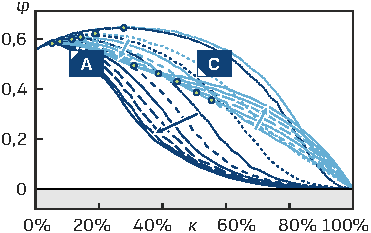
\includegraphics{content/bottleneck/images/tuev-engstelle-simulation-ergebnisse-kamo}%
\caption{Mittelwert über >>wahrscheinlichere<< Szenarien, konkret diejenigen in Abb.~\ref{fig:simparameterresults} die mit \textcolor{colorPRGreen}{$*$} markiert sind (d.h. $p\subs{f} < p\subs{b}$). Pfeile geben den Trend an, wie sich der Fluss über Erhöhung von $\tdmaxmax$ verändert. In dieser Abbildung sehen wir typische Effekte deutlicher: Erstens den Übergang \textbf{A} von einer anfänglichen Verschlechterung der >>Fairness<< bei niedrigen $\kappa$ hin zu einer Verbesserung; und zweitens für die >>nicht"=zählende<< Variante \ref{enum:non-counting} den Übergang von einer kurzen Phase in der $\tdmax$ die Fairness verbessert, hin zu einer dauerhaften Phase \textbf{C} in der $\tdmax$ den Verkehrsfluss systematisch zugunsten des freien Streifens beeinflusst. Dieses Problem vermeidet die >>zählende<< Variante \ref{enum:counting}. Im Gegensatz zu der Gesamtzahl aller Szenarien wie in Abb.~\ref{fig:simparameterresults} dargestellt tritt unter den hier gezeigten >>wahrscheinlicheren<< Szenarien keine nennenswerte Umkehr des Verkehrsflusses in Richtung des blockierten Streifens auf.}%
\label{fig:simparameterresults-accumulated}%
\end{figure}


%\subsection{Summary and Outlook}


%
%\begin{figure}
%\centering
%\includegraphics{images/tuev-kat-3.pdf}%
%\caption{Controlled preheating of the converter based on predicted waiting time \textbf{C} will assure $T_{\text{cat}} > T_{\min}$ \textbf{D} and reduce emission \textbf{E} on engine start.}%
%\vspace{-0.25cm}
%\end{figure}
%
%\begin{figure}
%\includegraphics[width=\columnwidth]{images/kat-fahrt2}%
%\caption{Both approaches are tested in real world traffic and in dynamometer tests with an automated test vehicle, using a test cycle of actual driving scenarios gathered on the Test Area Autonomous Driving Baden-Wuerrtemberg.}
%\label{}%
%\vspace{-0.4cm}
%\end{figure}







\subsection{Fazit und Ausblick}\label{sec:conclusion}


In diesem Beitrag haben wir betrachtet, welche diversen Aspekte bei der Entwicklung einer vernetzten Fahrfunktion eine Rolle spielen. Neben allgemeinen Erwägungen als Ausgangspunkt, zum Beispiel das Ziel einer >>evolutionären<< Erreichbarkeit immer höherer Durchsetzungsgrade, und dem Aspekt der Mensch"=Maschine"=Interaktion, haben wir besondere Aufmerksamkeit darauf gelegt, wie eine solche Funktion in der Simulation untersucht werden kann, und vor allem, warum Simulation für diese Fragen das Werkzeug der Wahl ist: Während Realexperimente für Teilaspekte wichtig und sinnvoll sind (und tatsächlich auch durchgeführt wurden, zum Beispiel zur Untersuchung von Funkreichweiten oder menschlichem Fahrverhalten), lässt sich die Wirkung in großen Maßstäben (d.h.: tausende oder hunderttausende Fahrzeuge und dauerhafter Betrieb) nicht in der Praxis studieren. Schon für einen Einzelversuch wären erhebliche Aufwände nötig -- und die Variation von menschlichem Verhalten ist so groß, dass ein Einzelversuch kaum repräsentativ wäre.


\fquot{}{Die Ergebnisse haben uns Einblicke in nicht"=offensichtliche Eigenschaften des Systems gegeben, die wir im Projekt auch tatsächlich nur dank der Simulationsergebnisse gefunden und verstanden haben.}{}

Die Simulation erlaubt uns dagegen die effiziente Durchleuchtung vielfältiger Parameterräume, und zwingt uns dazu, Annahmen transparent offenzulegen und diese in Wissenschaft und Technik durchaus auch kritisch zu diskutieren. Mit dem gewählten Modell konnten wir effizient $11\,016$ Parameterkombinationen über jeweils circa drei Tage simuliertem Verkehrsgeschehen abprüfen -- oder etwa 100 Jahren an unterschiedlichen Verkehrsszenarien. Und wir können mit einiger Sicherheit davon ausgehen, dass wir dadurch >>alle denkbaren<< Szenarien der Wirklichkeit zumindest näherungsweise betrachtet haben, was durch Realversuche schlicht unmöglich wäre.

Die Ergebnisse haben uns Einblicke in die Eigenschaften des entwickelten Systems (bzw. zwei seiner Varianten) gegeben, die von der reinen Spezifikation her nicht offensichtlich waren, und die wir im Projekt auch tatsächlich nur dank der Simulationsergebnisse gefunden und verstanden haben (und nicht durch systematische Überlegungen im Vorfeld). In diesem Sinne können Simulationen die Realität sicherlich nicht vollständig ersetzen (zumal in so reduzierter Modellierung), aber sie können helfen, wichtige Systemeigenschaften noch in frühen Entwicklungsphasen rechtzeitig zu verstehen.

Für die Entwicklung einer gesamten Fahrfunktion sind viele Facetten von Bedeutung, die wir hier nur ansatzweise beleuchtet haben -- auch, weil es nicht unser Ziel war, hier eine fertige Funktion für den Serieneinsatz zu entwickeln. Aber es zeigt, wie diverse Faktoren einen Einfluss haben, und wie man diesen Einfluss bemessen kann. Weitere Projektarbeiten finden sich zum Beispiel in \cite{naumann2017cooperativePlanning}, wo ein Ansatz dargestellt wird, auch in dünnem Verkehr Engstellen mithilfe vernetzter Fahrzeuge effizienter zu durchqueren. Welche Zeitlücken dabei von menschlichen Insassen akzeptiert werden, findet sich in \cite{ehrhardt2021gap}. Eine vollständigere Beschreibung der Untersuchungen dieses Beitrags findet sich in der Originalpublikation \cite{ziehn2023cooperative}.

Auch haben wir einige Vereinfachungen getroffen, die nicht allgemeingültig sind: Zum Beispiel nehmen wir an, dass ein balancierter Fluss optimal ist, bei dem in beide Fahrtrichtungen pro Stunde die gleiche Anzahl an Fahrzeugen abfließt. Wenn jedoch der \emph{Bedarf} in beide Richtungen unterschiedlich ist (zum Beispiel zur Rushhour nach Feierabend mit einem deutlich höherem Bedarf aus dem Stadtkern heraus als umgekehrt), dann ist ein >>ausgeglichener<< Fluss nicht unbedingt optimal. Eine tatsächliche Realisierung würde also auch den Bedarf berücksichtigen müssen.

Außerdem haben wir uns hier bewusst nicht damit befasst, welche >>Incentives<<, also Vorteile, die Insassen der vernetzten Fahrfunktion motivieren würden, diese häufiger und großzügiger einzusetzen. Wir haben lediglich und wie erwartet festgestellt, dass \emph{meistens} (!) ein großzügigerer Einsatz auch vorteilhaft für den Verkehrsfluss ist. Es ist also vorteilhaft, wenn die Insassen der vernetzten Fahrzeuge auch konkrete Vorteile bekommen, wenn sie die Funktion einsetzen -- beispielsweise Tank- oder Laderabatte.

Schließlich ist festzuhalten, dass sich die Entwicklung eines solchen Systems nie rein auf eine einzelne Simulationsstudie stützen sollte. Realexperimente sowie komplexere Simulationen können unter ausgewählten Parametern prüfen, ob die hier vorgestellte Simulation zu denselben Ergebnissen kommt, und ob Effekte auftreten, die aus dem vereinfachten Simulationsmodell nicht hervorgehen. Nur das Zusammenspiel unterschiedlicher Methoden kann ein belastbares Bild davon abgeben, ob eine zukünftige Fahrfunktion >>gut<< oder >>schlecht<< ist -- mit dem gemeinsamen Ziel, den Unterschied zuverlässig festzustellen bevor das System in den Markt, oder auch nur in die Serienentwicklung kommt. \markEndOfContent





\nocite{ziehn2023cooperative}

\printbibliography[heading=subbibliography]
